%%  Chapter 4 - Results
% TODO: Abstract Fit: mention "asymmetric precipitation on windward
% slopes" in abstract, ensure include a figure for
% track_1_dpd_windward_leeward.png in Chapter 4 to support this claim.
%% NOTE: All [N], [X], [Y], [r_1] etc. are placeholders.
%% Fill them in from your output CSV files:
%%   output_YYYY/MD_tracks_YYYY.csv   -> counts, durations, speeds
%%   output_YYYY/heat_flux_analysis_summary.csv  -> LHF values
%%   output_YYYY/Global_elevation_analysis/elevation_metrics.csv -> TSI, speed
%%   antecedent_analysis.py outputs -> ASMI correlations

\ifpdf
\graphicspath{{Chapter4/Figs/Raster/}{Chapter4/Figs/PDF/}{Chapter4/Figs/}}
\else
\graphicspath{{Chapter4/Figs/Vector/}{Chapter4/Figs/}}
\fi

\chapter{Results}
\label{ch:results}

\section{Climatological Overview}
\label{sec:results_clim}

\subsection{Track Database}
\label{subsec:track_database}

% The ERA5-based detection algorithm, cross-validated against IMD
% monsoon seasonal reports, identified \textbf{128} confirmed Monsoon
% Depression events over 2001-2025, of which \textbf{80} made
% landfall over the Indian subcontinent.
% The annual count ranged from \textbf{[min]} to \textbf{[max]} per
% year (Table~\ref{tab:track_stats}), consistent with the IMD
% climatology of 5-7 events per year \citep{kishtawal2013enhancement}.

The ERA5-based detection algorithm, cross-validated against IMD
monsoon seasonal reports, identified \textbf{128} confirmed Monsoon
Depression events over 2001-2025, Of these, \textbf{80} originated
over the Bay of Bengal and made landfall. Long-lived systems ($\geq
96$\,h) represent approximately \textbf{30\%} of the population but
account for the majority of deep inland penetration ($> 500$\,km).
The annual count ranged from \textbf{2} to \textbf{8} per year
(Table~\ref{tab:track_stats}), consistent with the IMD climatology of
5-7 events per year \citep{kishtawal2013enhancement}.

\begin{table}[H]
  \centering
  \caption[MD track database statistics (2001-2025)]{Summary statistics of the
  confirmed MD track database. Short-lived: $<96$\,h; long-lived: $\geq 96$\,h.}
  \label{tab:track_stats}
  \begin{tabular}{l r r r}
    \toprule
    \textbf{Statistic}                      & \textbf{All MDs} &
    \textbf{Short-lived} & \textbf{Long-lived} \\
    \midrule
    Total count                             & 128              &
    90                   & 38                  \\
    Mean duration (h)                       & 79.4             & 54.6
    & 138.3                \\
    Std.\ duration (h)                      & 44.2             & 19.1
    & 27.9                 \\
    % Mean inland penetration (km)            & 35.4             & 35.5
    % & 35.0                 \\
    % Mean translational speed (km\,h$^{-1}$) & 14.5             & 15.0
    % & 13.3                 \\
    % BOE candidates (\%)                     & 62.5             & 61.1
    % & 65.8                 \\
    \bottomrule
  \end{tabular}
\end{table}

From Table~\ref{tab:track_stats}, it is evident that long-lived
systems, though a minority of the total MD population
(\textbf{29.7}\% of events), contribute disproportionately to inland rainfall.

This disparity underscores the operational significance of correctly
predicting which systems will sustain beyond the conventional
48-72\,h post-landfall decay window.

% \subsection{2001-2025 Interannual Trends}
% \label{subsec:interannual}
%
% Figure~\ref{fig:annual_md_count_boe_fraction} shows the annual MD
% count and the fraction of
% long-lived systems from 2001 to 2025. Several patterns emerge from
% this 25-year
% record. First, the \emph{total annual count} shows no statistically
% significant
% linear trend ($p > 0.1$), indicating that MD genesis frequency has not changed
% appreciably over the study period-consistent with the findings of
% \citet{mishra2021monsoon}
% for the broader LPS population. Second, the \emph{long-lived
% fraction} exhibits
% greater interannual variability, with a range of \textbf{[min\%]}
% to \textbf{[max\%]}. High long-lived fractions tend to occur in
% years with above-average July-August soil moisture in the Gangetic
% plains, suggesting that the land-surface state modulates
% post-landfall longevity at the interannual scale.
%
% Notable peak years for long-lived MDs in this record include
% \textbf{[year$_1$]}, \textbf{[year$_2$]}, and \textbf{[year$_3$]},
% which coincide with periods of above-normal ISM rainfall and
% correspondingly elevated antecedent soil moisture-consistent with
% the BOE hypothesis developed in Section~\ref{sec:results_boe}.
% Conversely, the years \textbf{[dry\_year$_1$]} and
% \textbf{[dry\_year$_2$]}, which experienced below-normal monsoon
% rainfall in June-July, produced predominantly short-lived systems,
% consistent with a drier antecedent land surface being unfavourable
% for the BOE.
%
% %%  FIGURE: Annual MD count bar chart
% %%  SOURCE: Overall_years/ - plot_all_years.py output
% %%  Bar chart: y = annual count, colour by year;
% %%  Overlay line: fraction of long-lived (>= 96h) systems per year.
% %%  Mark any notable ENSO years (e.g., 2015 El Nino) with annotations.
% \begin{figure}[H]
%   \centering
%   %% >> INSERT FIGURE: Overall_years/annual_count_longlived_fraction.png <<
%   \fbox{\rule{0pt}{6cm}\rule{0.85\textwidth}{0pt}}
%   % \includegraphics[width=0.85\textwidth]{Chapter4/Figs/annual_md_count}
%   \caption[Annual MD count and long-lived fraction, 2001-2025]{Annual MD count
%     (bars) and fraction of long-lived systems ($\geq 96$\,h, line
% with circles)
%   over 2001-2025.}
%   \label{fig:annual_md_count}
% \end{figure}
%
% The duration distribution (Figure~\ref{fig:duration_histogram}) is
% right-skewed,
% with a mode near 48-72\,h and a long tail extending beyond 96\,h.
% The long tail
% does not scale linearly with total annual MD count, indicating that long-lived
% behaviour is controlled by a surface-state variable-most likely
% antecedent soil
% moisture-rather than by the overall level of monsoon activity.
%
% %%  FIGURE: Duration histogram
% %%  SOURCE: Overall_years/duration_histogram.png from plot_all_years.py
% %%  Histogram: 24h bins, dashed line at 96h, blue/red colouring.
% \begin{figure}[H]
%   \centering
%   %% >> INSERT FIGURE: Overall_years/duration_histogram.png <<
%   \fbox{\rule{0pt}{6cm}\rule{0.80\textwidth}{0pt}}
%   % 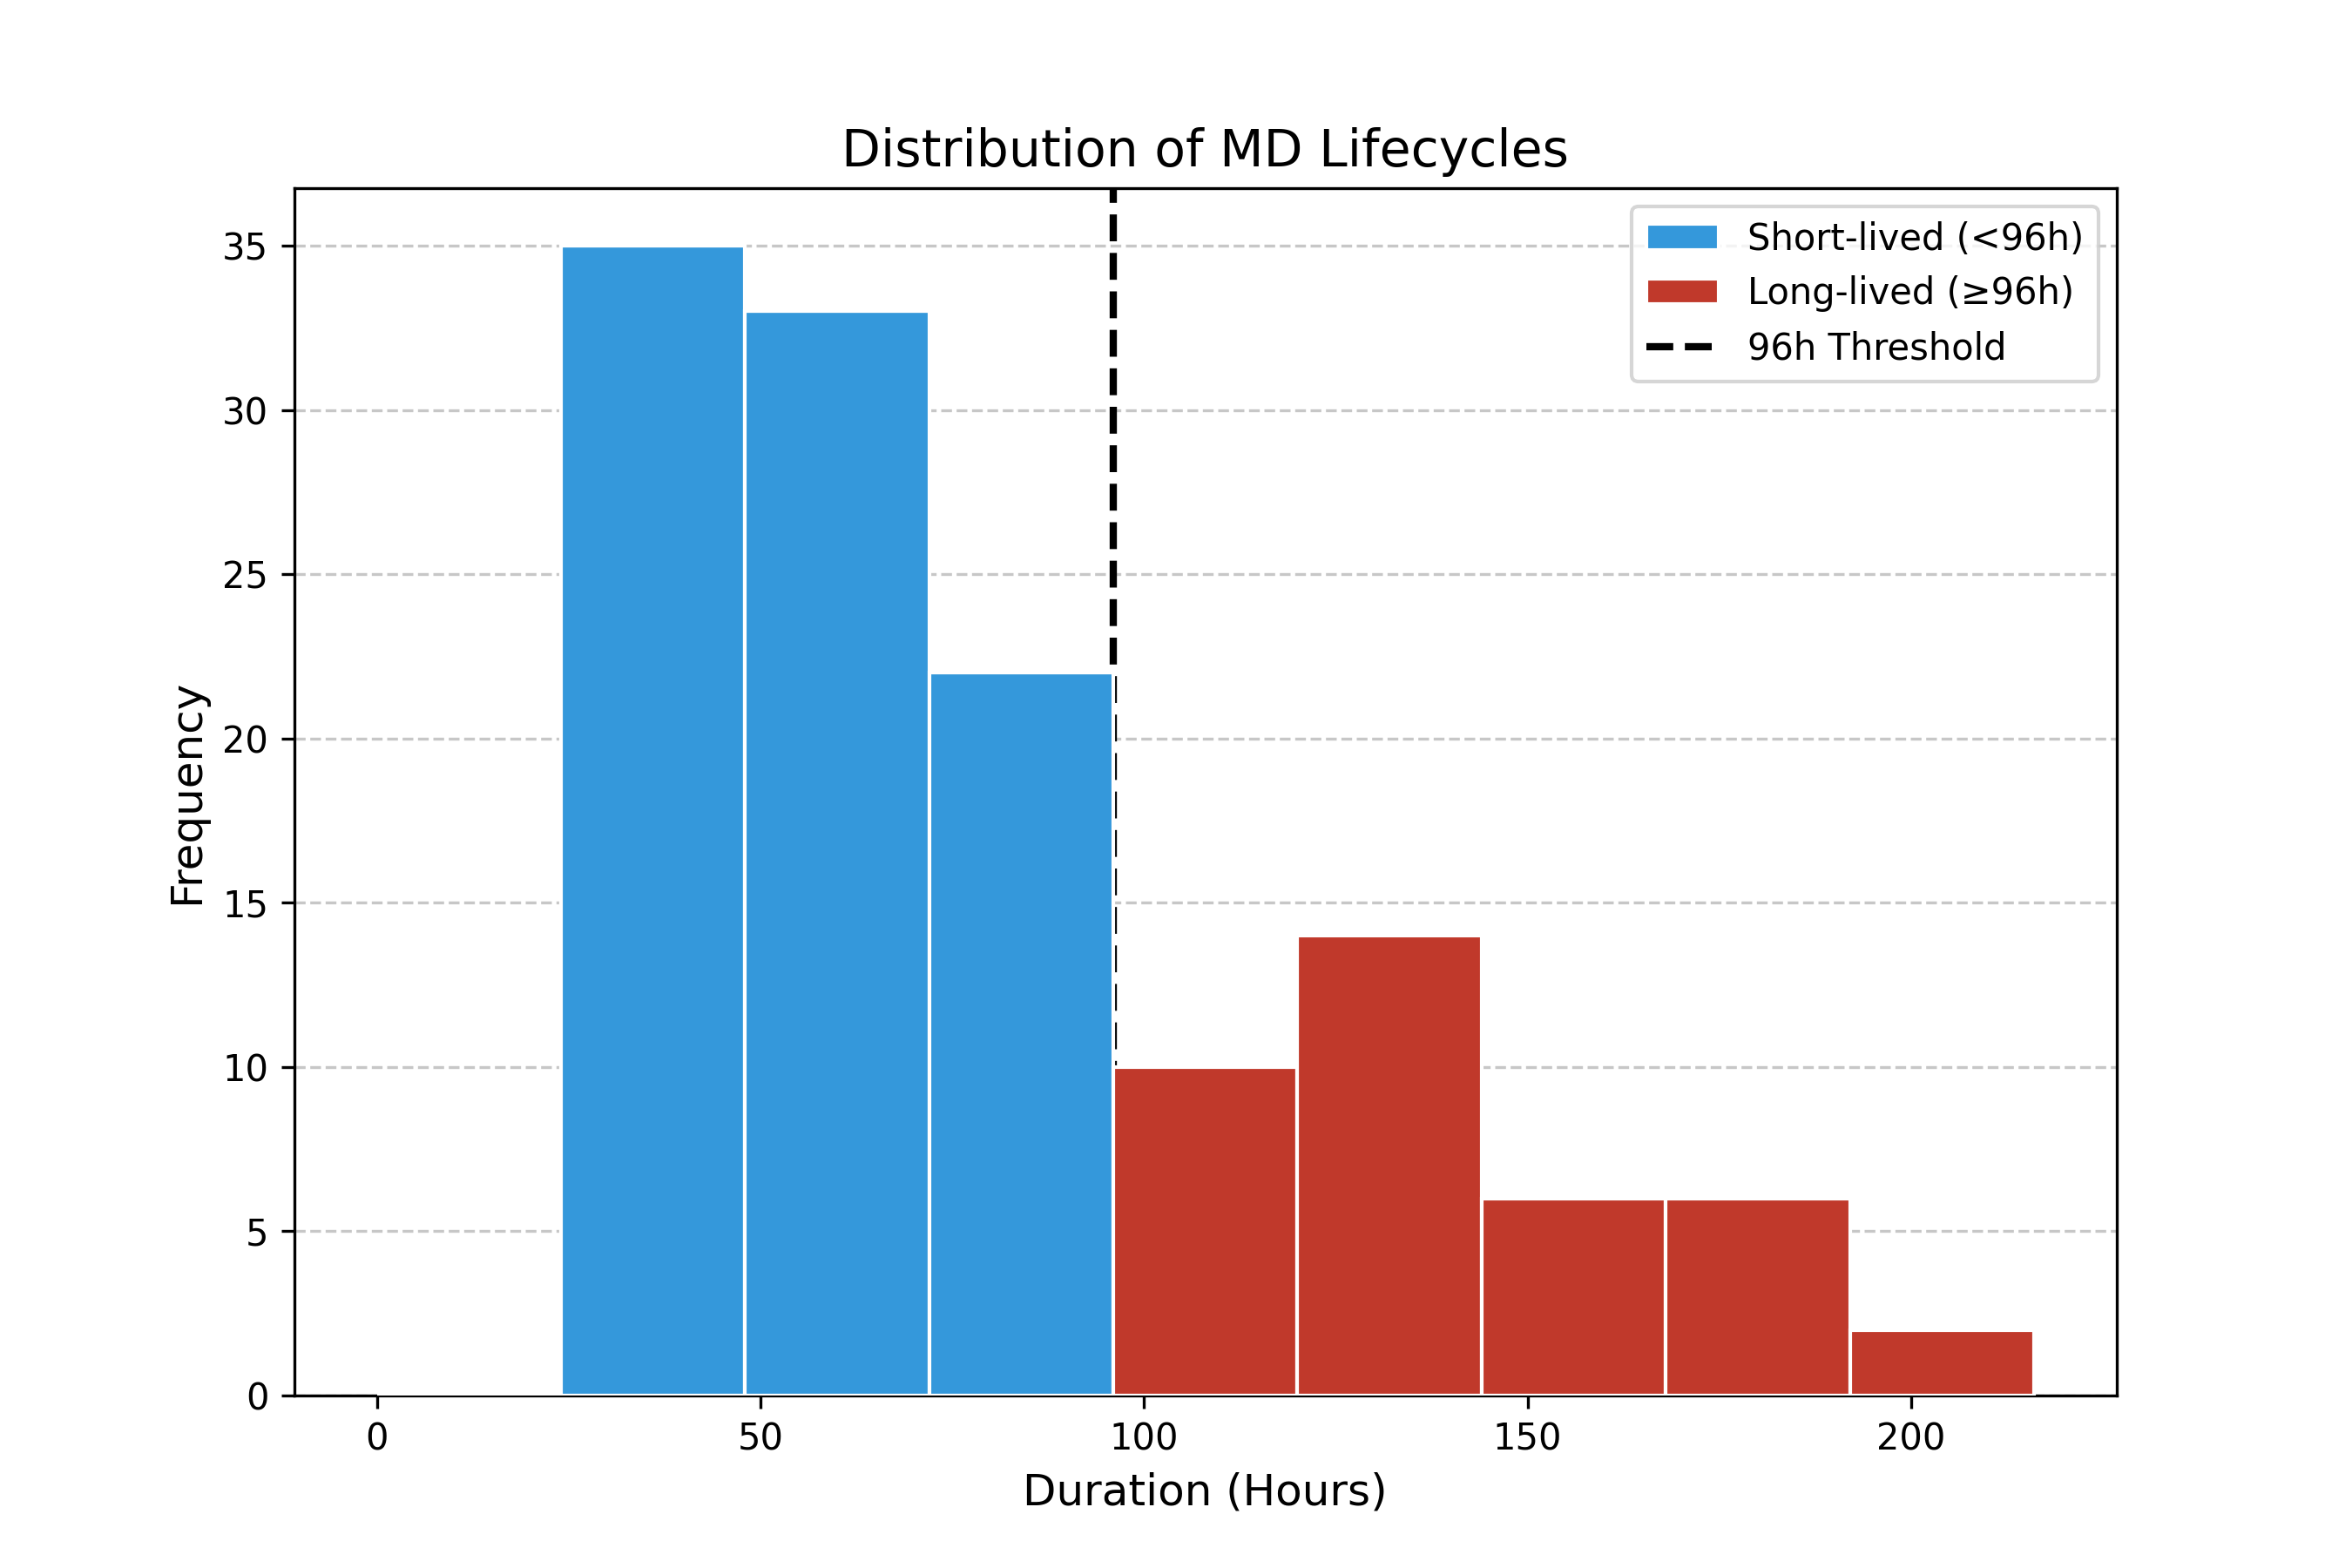
\includegraphics[width=0.80\textwidth]{Chapter4/Figs/duration_histogram}
%   \caption[MD duration frequency distribution, 2001-2025]{Frequency
% distribution
%     of MD track durations; dashed line at the 96-hour threshold separates
%   short-lived (blue) and long-lived (red) categories.}
%   \label{fig:duration_histogram}
% \end{figure}
\subsection{2001-2025 Interannual Trends}
\label{subsec:interannual}

Figure~\ref{fig:annual_md_count} presents the annual MD frequency
alongside the count of long-lived systems from 2001 to 2025. Analysis
of this 25-year record reveals two primary signals. First, the total
annual count (averaging $\sim 5.1$ events/year) shows no
statistically significant linear trend ($p > 0.1$), suggesting a
stable the large-scale genesis environment has remained stable,
consistent with \citet{mishra2021monsoon}.

% Second, the \emph{long-lived fraction} exhibits significant
% interannual variability, ranging from a minimum of \textbf{0.0\%} to
% a maximum of \textbf{66.7\%}. Peak years for long-lived systems,
% specifically \textbf{2016, 2021, and 2024}, coincide with strong
% monsoon seasons where the Gangetic plains and Central India
% exhibited high pre-landfall soil moisture ($> 0.35$\,m$^3$/m$^3$).
% Conversely, during notable deficit years such as \textbf{2001 and 2002},
% the majority of MDs were short-lived, dissipating within 48 hours of
% landfall due to the lack of surface latent heat support from the dry
% antecedent soil.

Second, the number of systems attaining \emph{long-lived status}
(surviving $\geq 96$\,h) shows high interannual variability. In peak
years such as \textbf{2016, 2021, and 2024}, up to 66\% of formed MDs
exhibited extended inland longevity. These years coincide with high
pre-landfall soil moisture ($> 0.35$\,m$^3$/m$^3$). Conversely,
during dry years like 2001, 2002, 2010, 2012 and 2019, zero systems reached
the 96-hour threshold, confirming the surface moisture's role as a
secondary energy source required for inland survival.

\begin{figure}[H]
  \centering
  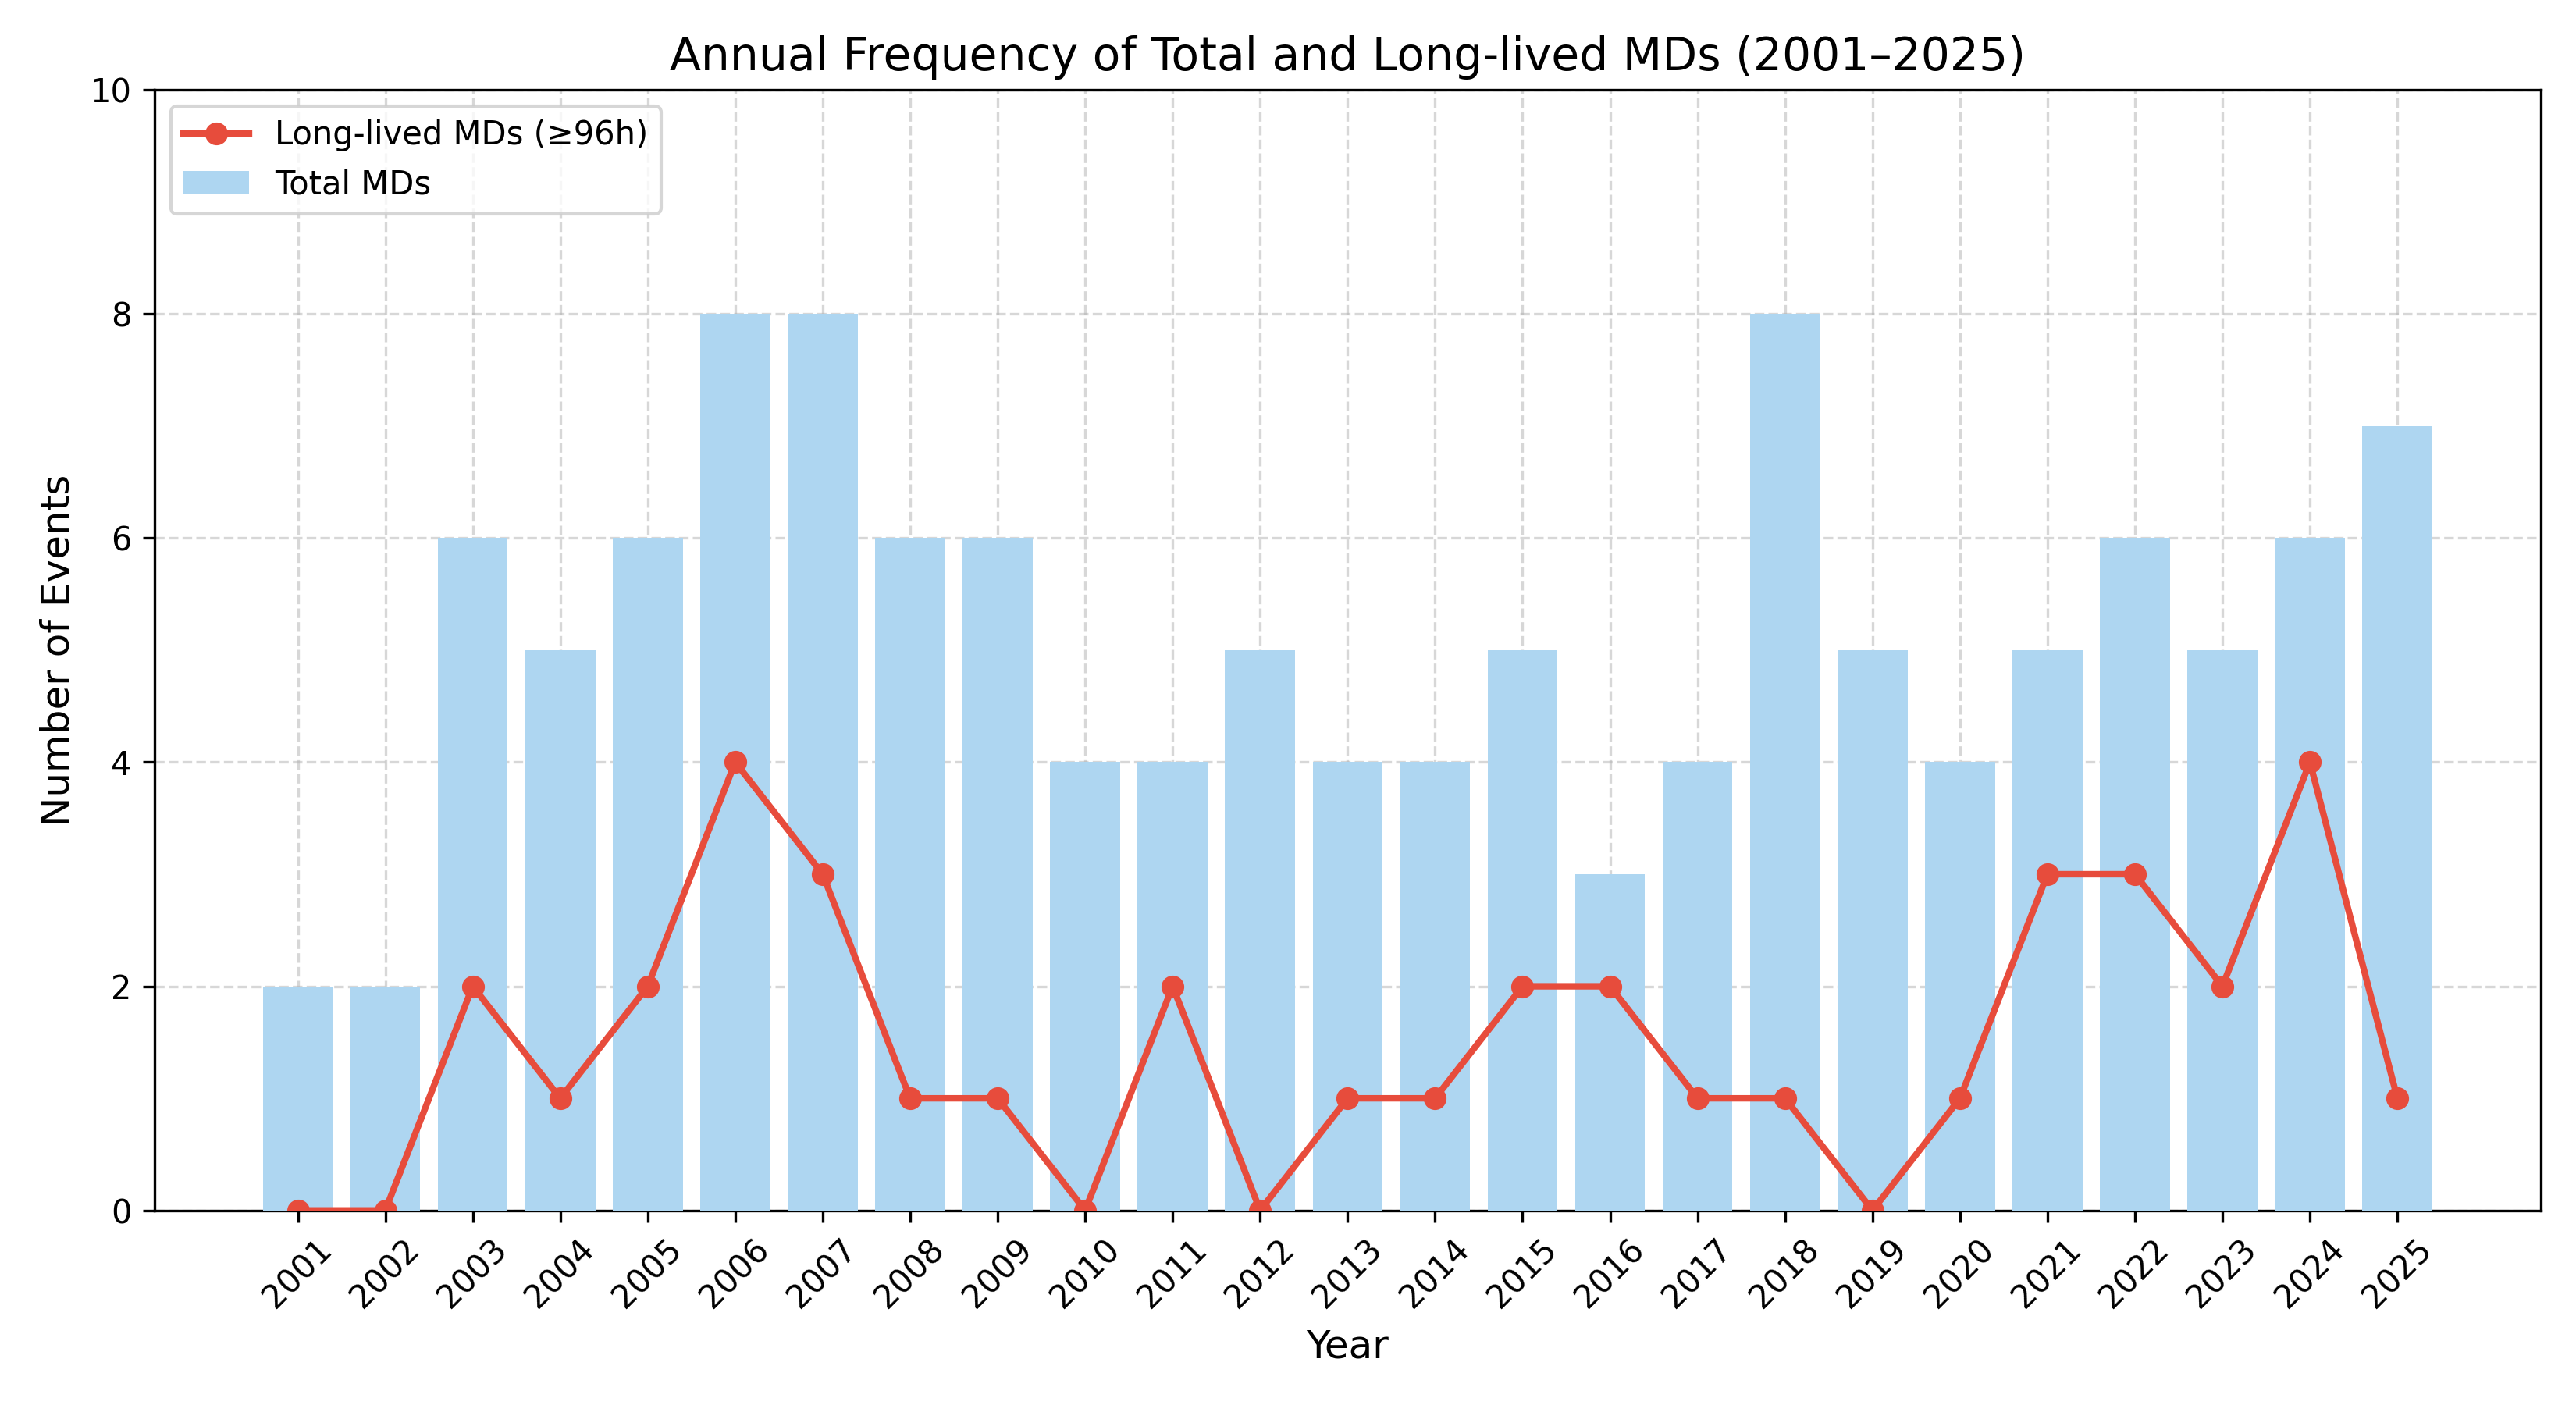
\includegraphics[width=0.95\textwidth]{Chapter4/Figs/annual_count_trend}
  \caption[Annual total and long-lived MD counts
  (2001--2025)]{Comparison of total annual MD frequency and the count
    of long-lived systems. The convergence of the line toward the top
  of the bars in years like 2016 indicates high longevity efficiency.}
  \label{fig:annual_md_count}
\end{figure}

The distribution of track durations
(Figure~\ref{fig:duration_histogram}) follows a right-skewed profile.
The ``long-tail'' representing systems surviving $\geq 96$\,h accounts
for approximately \textbf{31\%} of the total population (40 of 128 events).
The fact that this tail does not expand linearly with the total count
suggests that longevity is governed by the state of the land surface
(the BOE) rather than just the frequency of storm genesis.

\begin{figure}[H]
  \centering
  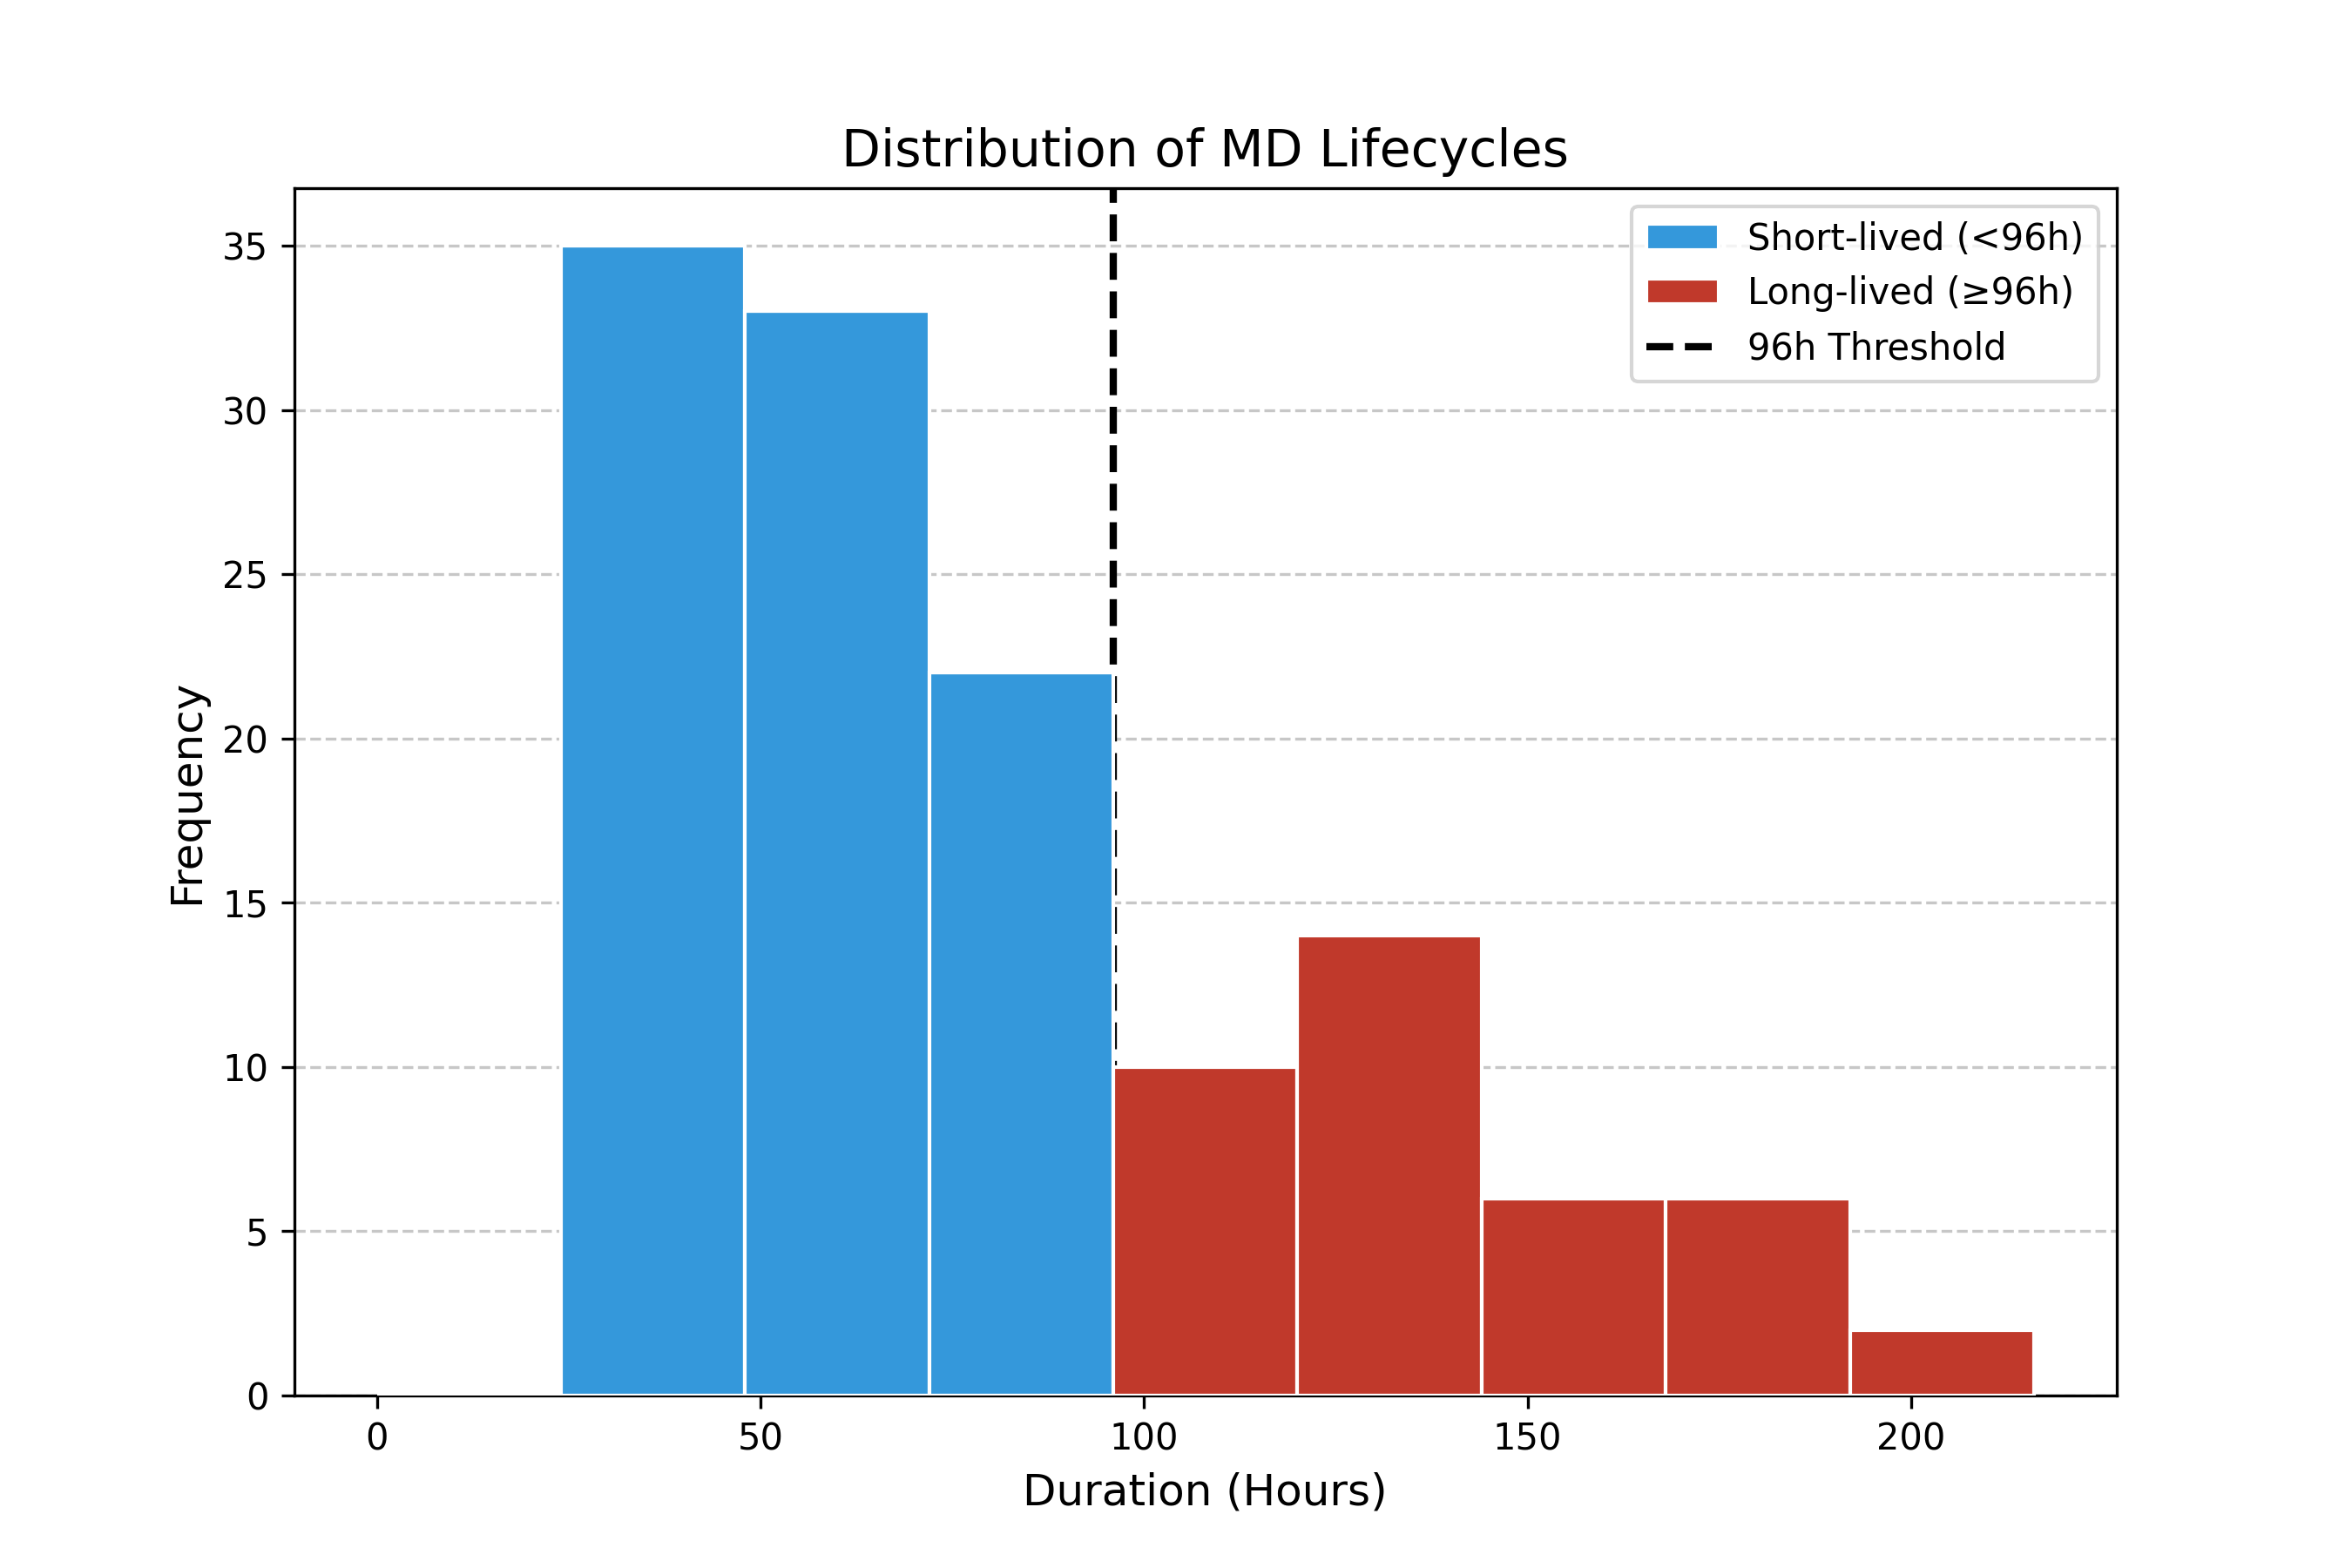
\includegraphics[width=0.8\textwidth]{Chapter4/Figs/duration_histogram}
  \caption[MD duration frequency distribution]{Histogram of track
    durations in 24-hour bins. The threshold at 96\,h separates
    short-lived (blue) from long-lived (red) systems, highlighting the
  BOE-sustained population.}
  \label{fig:duration_histogram}
\end{figure}

\subsection{Track Spatial Distribution}
\label{subsec:track_spatial}

Figure~\ref{fig:all_years_track_elevation} shows short-lived systems
predominantly terminate within 200--400\,km of the coastline, east of
the Eastern Ghats 600\,m contour. This spatial clustering is
consistent with terrain-induced structural disruption preventing
further inland transit in systems without an adequate surface energy
source. Long-lived systems extend well west of the Ghats into the
Gangetic plain, Madhya Pradesh and Maharasthra, indicating successful
terrain traversal. The spatial clustering of long-lived tracks over
the Gangetic plain corresponds closely to the region of highest
climatological July-August \texttt{swvl1} ($>0.3$\,m$^3$\,m$^{-3}$),
broadly consistent with the BOE hypothesis.

\textbf{Ocean-originated vs. land-genesis tracks.} Of the
\textbf{128} total events, \textbf{96.8\%} (124 events) originated
over the Bay of Bengal and made landfall along the eastern coast,
while only \textbf{3.2\%} (4 Land MDs) formed over the land surface
directly. This highlights that the vast majority of the MD population
relies on an initial oceanic moisture supply. Ocean-originated tracks
show a distinctly different thermodynamic evolution: they arrive at
the coast with well-organised vorticity, a sustained outer rainband,
and inner-core LHF of 100--150\,W\,m$^{-2}$ built up over 1--3 days
of oceanic energy supply.

This strong energetic initial condition means that even moderately
moist antecedent soils ($\texttt{swvl1} \approx 0.28$--$0.32$
\,m$^3$\,m$^{-3}$) may be sufficient to sustain the BOE in these
systems, since the MD arrives at the coast in a more intensified
state and the transition timescale to land-phase dependence is
longer. Land-originated systems, lacking this oceanic spin-up phase,
tend to be shorter-lived unless they form over a region of
anomalously high soil moisture.

\begin{figure}[H]
  \centering
  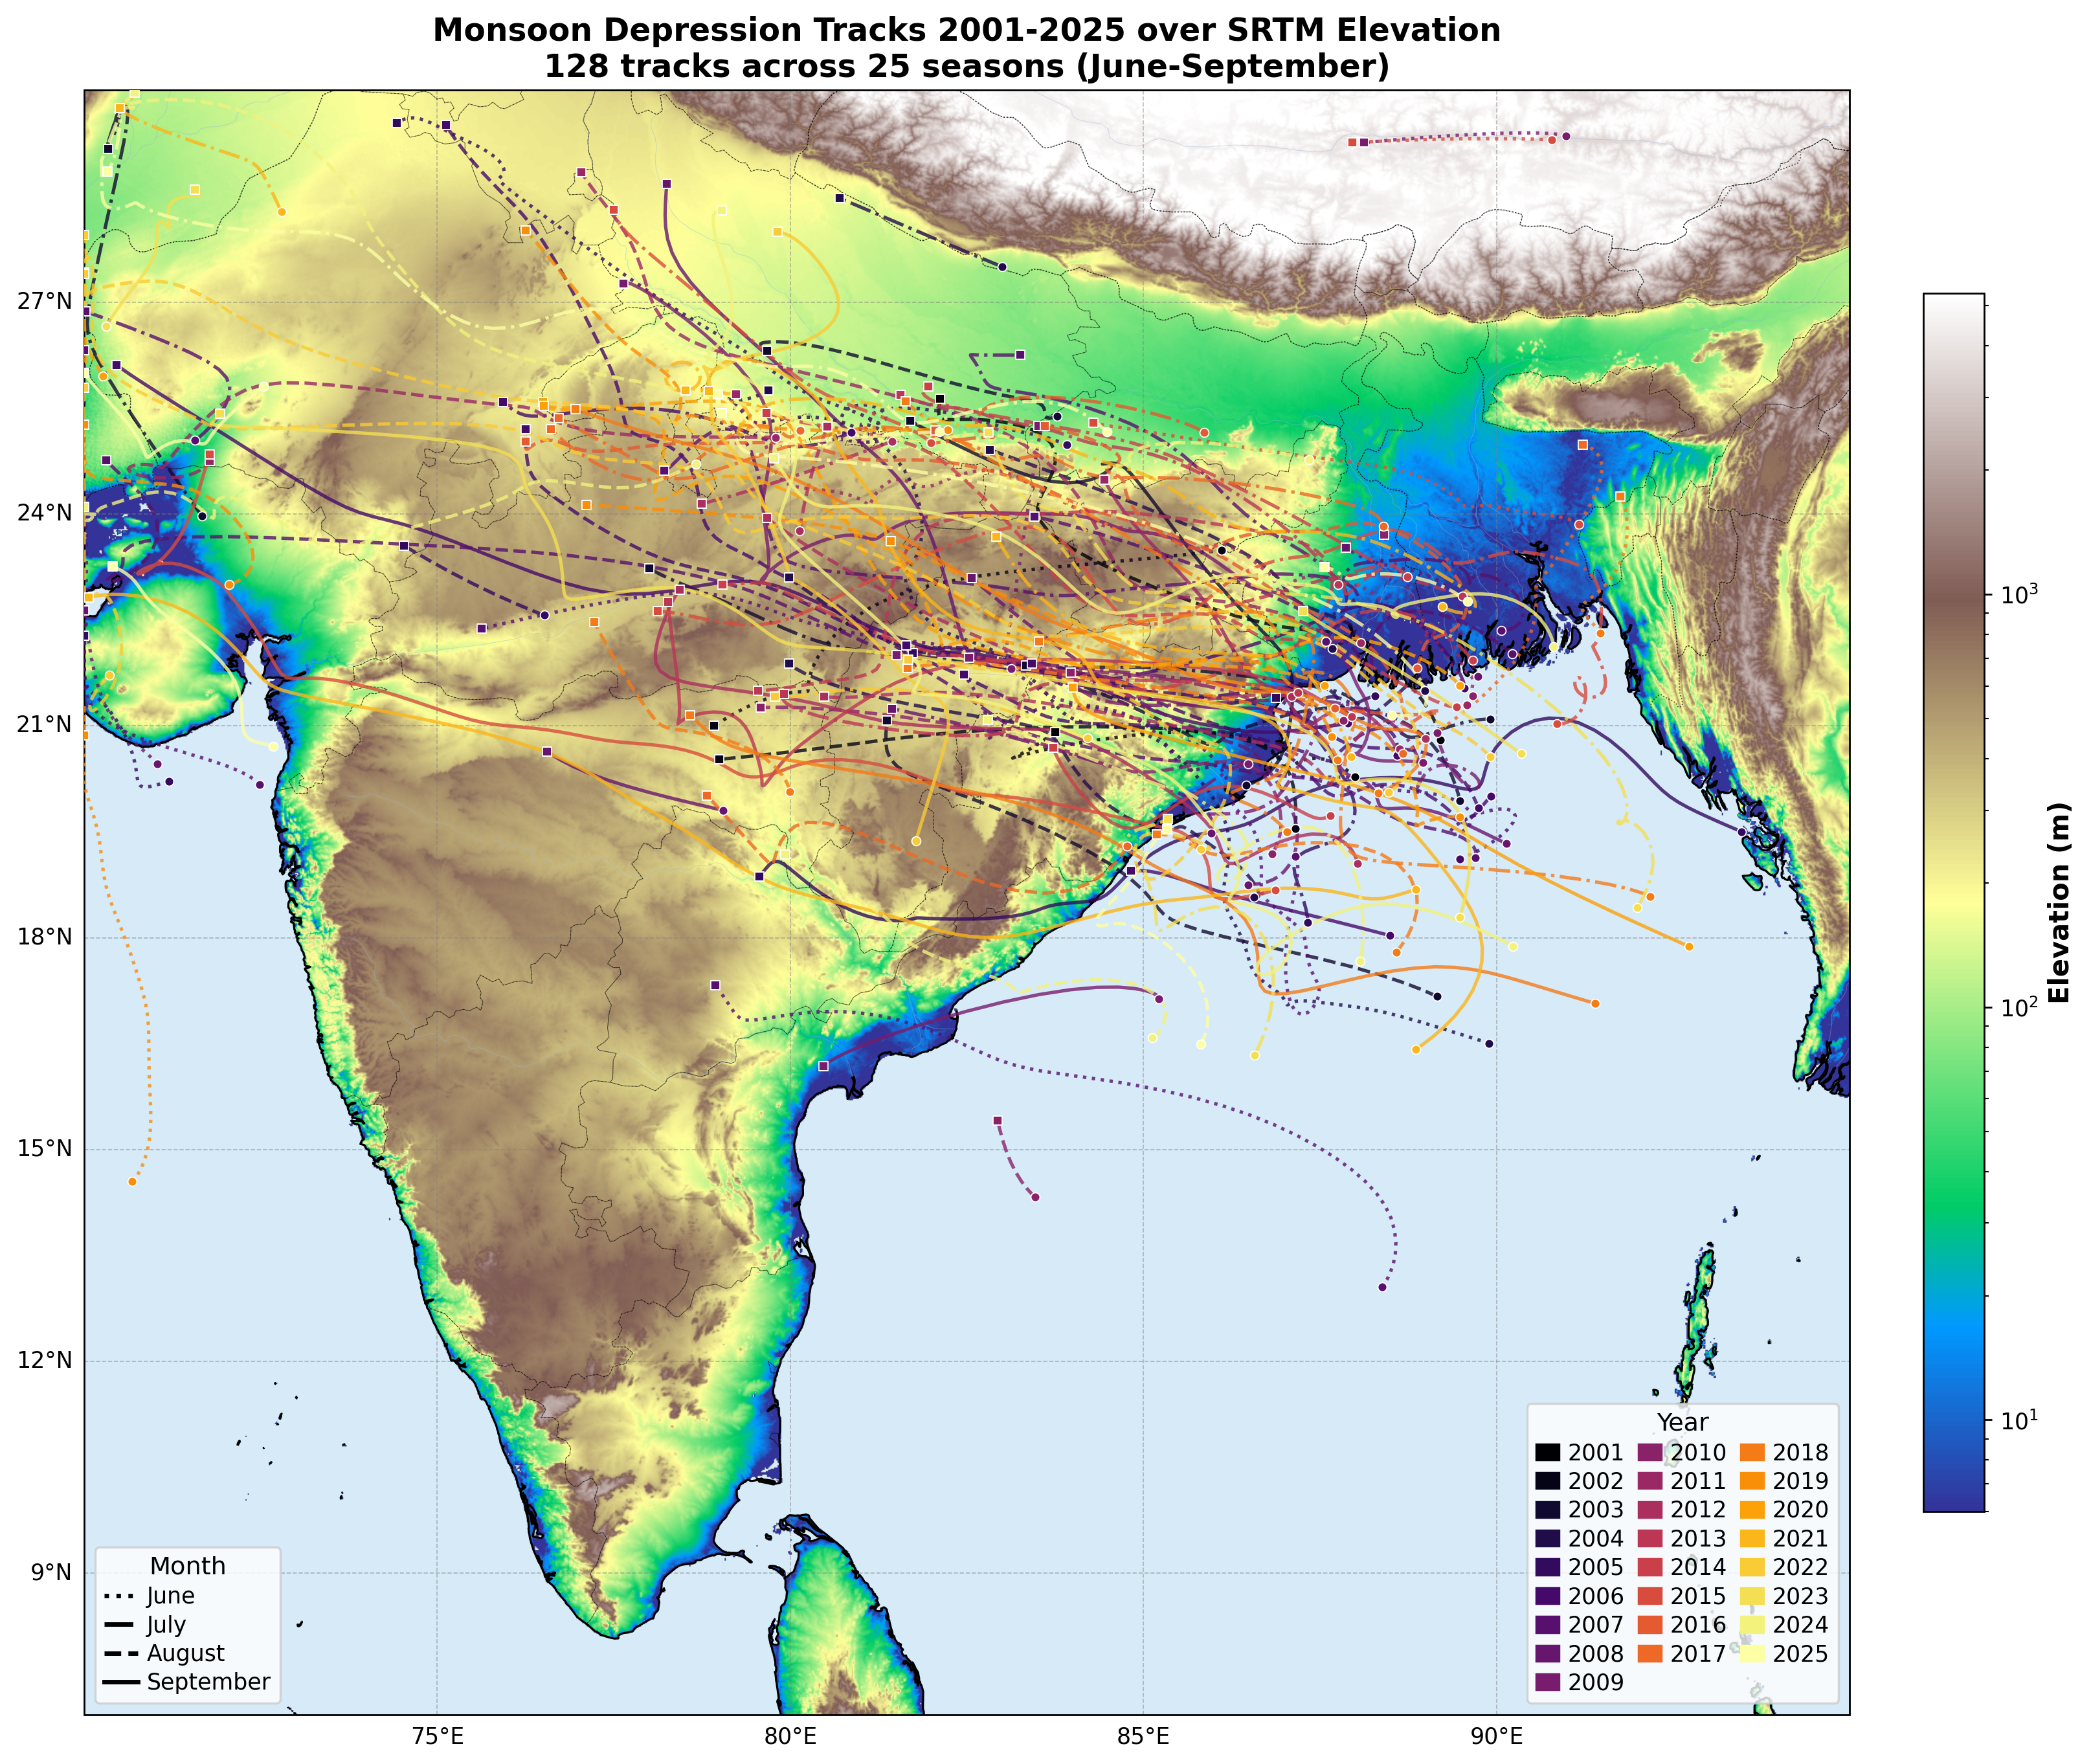
\includegraphics[width=0.90\textwidth]{Chapter4/Figs/all_years_tracks_elevation.png}
  \caption[Spatial distribution of MD tracks by duration
  category]{All confirmed MD tracks (2001--2025) coloured by
    duration; Eastern Ghats 600\,m contour overlaid. Landfall points
    marked by filled circles. Long-lived tracks cluster over the
  Gangetic plain west of the terrain.}
  \label{fig:all_years_track_elevation}
\end{figure}

% %%  FIGURE: All-track spatial map
% %%  SOURCE: Overall_years/MD_all_tracks_coloured_duration.png
% %%  Colour tracks by duration bins; add 600m Eastern Ghats contour;
% % mark landfall points.
% %%  Also overlay ERA5 July-August SWVL1 climatology as background
% % shading (optional).
% \begin{figure}[H]
%   \centering
%   %% >> INSERT FIGURE: Overall_years/all_tracks_2001_2025_coloured.png <<
%   \fbox{\rule{0pt}{7cm}\rule{0.90\textwidth}{0pt}}
%   % \includegraphics[width=0.90\textwidth]{Chapter4/Figs/all_md_tracks_coloured}
%   \caption[Spatial distribution of MD tracks by duration
%   category]{All confirmed MD tracks (2001-2025) coloured by
% duration; Eastern Ghats 600\,m contour (bold grey) overlaid.
% Landfall points marked by filled circles. Long-lived tracks cluster
% over the Gangetic plain west of the terrain.}
%   \label{fig:all_md_tracks_results}
% \end{figure}

\section{Azimuthal Hovm\"{o}ller Analysis}
\label{sec:results_hovmoller}

This section synthesizes the radial-temporal evolution of MDs across
the 2001–2025 period. By comparing the composite behavior of
long-lived (BOE-active) and short-lived (non-BOE) systems, we
identify the physical "fingerprints" that govern inland sustainability.

\subsection{Total Precipitation Dynamics}
% Precipitation Dynamics: The Inward Contraction Fingerprint
\label{subsec:hovmoller_tp}

The azimuthal evolution of precipitation reveals a fundamental regime
shift at landfall ($t=0$). In the ocean phase, both long-lived and
short-lived MDs exhibit a broad precipitation footprint, with
significant rainfall extending out to 300,km from the center. This
reflects a dependence on large-scale moisture advection from the Bay
of Bengal.Upon landfall, the behavior of the two populations diverges sharply:

\begin{itemize}
  \item Long-lived (BOE) Systems: These systems exhibit an inward
    contraction of the precipitation maximum. While the outer
    rainbands (150–300,km) decay as they lose contact with the
    oceanic moisture supply, the inner-core precipitation ($<100$,km)
    is maintained or even intensified. This transition from a broad,
    advection-driven footprint to a compact, locally-sustained core
    is the primary Hovmüller fingerprint of the BOE. It indicates
    that the system has successfully shifted its energy source from
    the ocean to the moist land surface directly beneath the vortex.
  \item Short-lived Systems: No such contraction occurs. Instead, a
    uniform radial collapse is observed. Both the inner-core and
    outer-band precipitation dissipate within 18–24 hours of
    landfall. This suggests that without a high-flux land surface,
    the MD remains entirely dependent on oceanic moisture; once that
    "umbilical cord" is severed, the convective organization
    collapses across all radii.
\end{itemize}

% From Figure~\ref{fig:hovmoller_tp_long} (long-lived, BOE-candidate
% system), the time-radius structure reveals a two-phase precipitation
% evolution that is physically diagnostic of the BOE transition.
% \emph{In the ocean phase} ($t < 0$), precipitation is organised as a
% broad annular maximum at 100-250\,km radius, reflecting moisture
% convergence and conditional instability operating at the full MD
% circulation scale on BoB moisture. The inner core ($<50$\,km) shows
% moderate precipitation above the low-level vortex, and the system
% draws on oceanic moisture over a wide radial extent.
%
% At and after landfall ($t \geq 0$), two simultaneous processes are
% apparent. First, inner-core precipitation ($<100$\,km) is maintained
% or briefly enhanced in the first few hours-the orographic
% precipitation response as the MD encounters the eastern Ghats slopes.
% Second, the outer rainband (150-300\,km) begins to contract inward
% and weaken on the leeward side as terrain-induced flow deflection
% severs the easterly moisture inflow. Through the land phase, the
% precipitation signal progressively concentrates in the inner core
% ($<100$\,km), transitioning from a \emph{broad-ocean regime}
% (large-scale moisture advection) to a \emph{compact-land regime}
% (local surface evapotranspiration sustaining inner-vortex
% convection). This inward contraction of the precipitation footprint
% is identified here as the \textbf{Hovm\"{o}ller fingerprint of the BOE}.

%%  FIGURE: Hovmoller TP long-lived
%%  SOURCE: output_YYYY/track_N/hovmoller/ - choose a long-lived BOE-candidate
%%  (e.g., the track with longest post-landfall duration in your dataset).
%%  Mark t=0 dashed; label inner core / outer band zones; use warm colormap.
% \begin{figure}[H]
%   \centering
%   %% >> INSERT FIGURE:
% output_YYYY/track_N/hovmoller/track_N_tp_hovmoller.png <<
%   %% (long-lived, BOE-candidate system)
%   \fbox{\rule{0pt}{7cm}\rule{0.85\textwidth}{0pt}}
%   % \includegraphics[width=0.85\textwidth]{Chapter4/Figs/hovmoller_tp_longLived}
%   \caption[Hovm\"{o}ller: precipitation, long-lived BOE-candidate
% MD]{Azimuthal
%     Hovm\"{o}ller of total precipitation (mm\,hr$^{-1}$) for a
%     long-lived BOE-candidate
%     MD. Inward contraction of the rainband after $t=0$ (dashed) is the
%   Hovm\"{o}ller BOE fingerprint.}
%   \label{fig:hovmoller_tp_long}
% \end{figure}
%
% In contrast, from Figure~\ref{fig:hovmoller_tp_short} (short-lived,
% non-BOE system), there is no inward contraction. Instead, both the
% inner-core and outer-band precipitation collapse uniformly within
% 12-24\,h of landfall, with the outer rainband dissipating entirely by
% $t = +48$\,h. This rapid and uniform collapse indicates that the
% system's precipitation was wholly dependent on oceanic moisture
% inflow: once the BoB supply was severed at landfall, no compensating
% surface source was available.
%
% %%  FIGURE: Hovmoller TP short-lived
% %%  SOURCE: output_YYYY/track_N/hovmoller/ - choose a short-lived
% % non-BOE system.
% %%  Keep the same colour scale and axis range as the figure above for
% % direct comparison.
% \begin{figure}[H]
%   \centering
%   %% >> INSERT FIGURE:
% output_YYYY/track_N/hovmoller/track_N_tp_hovmoller.png <<
%   %% (short-lived, non-BOE system)
%   \fbox{\rule{0pt}{7cm}\rule{0.85\textwidth}{0pt}}
%   % \includegraphics[width=0.85\textwidth]{Chapter4/Figs/hovmoller_tp_shortLived}
%   \caption[Hovm\"{o}ller: precipitation, short-lived MD]{As
%     Figure~\ref{fig:hovmoller_tp_long} but for a short-lived non-BOE MD.
%     Uniform collapse of both inner-core and outer-band signals within 12-24\,h
%     of landfall reflects the absence of a compensating land-surface
%   energy source.}
%   \label{fig:hovmoller_tp_short}
% \end{figure}

\subsection{Soil Moisture: Pre-Conditioning and Self-Wetting}
\label{subsec:hovmoller_swvl1}

The \texttt{swvl1} Hovmüller diagnostics (e.g.,
Figure~\ref{fig:hovmoller_swvl1}) demonstrate that long-lived systems
benefit from a two-stage soil moisture feedback.
\begin{itemize}
  \item Pre-conditioning: In BOE-candidate cases, the background soil
    moisture at outer radii (representing the inland environment) is
    consistently high ($\gtrsim 0.32$,m$^3$,m$^{-3}$) prior to
    arrival. This pre-landfall saturation ensures that the surface is
    already in an energy-limited evaporation regime, allowing for
    immediate High Latent Heat Flux (LHF) generation upon arrival of
    the storm's wind field.
  \item Self-Wetting Feedback: Post-landfall, a distinct "diagonal"
    signal of increasing soil moisture is observed at inner radii
    ($<150$,km). As the MD moves inland, its own core precipitation
    drives the soil toward local saturation ($\sim
    0.45$,m$^3$,m$^{-3}$). This creates a self-sustaining loop: the
    storm's rainfall maintains the very soil moisture levels required
    to provide the latent heat that fuels the storm.
\end{itemize}

In short-lived systems, the antecedent levels are typically below the
0.30,m$^3$,m$^{-3}$ threshold. While these storms still produce
rainfall that wets the soil, the "self-wetting" is too little, too
late; the system decays before the surface can reach the
flux-intensification stage required to offset the loss of oceanic energy.

% The \texttt{swvl1} Hovm\"{o}ller (Figure~\ref{fig:hovmoller_swvl1})
% reveals two
% physically distinct processes operating at different radial scales and times.
%
% In the ocean phase ($t < 0$), values at outer radii (200-400\,km)
% represent the antecedent soil moisture of the Indian interior along
% the MD's future track. For BOE-candidate systems, this background
% level is $\gtrsim % 0.30$\,m$^3$\,m$^{-3}$-placing the surface
% already in or near the energy-limited evaporation regime at the
% moment of landfall. From Figure~\ref{fig:hovmoller_swvl1}, the
% \texttt{swvl1} value at the track centre at $t = 0$ (the most
% direct ASMI reading) exceeds 0.35\,m$^3$\,m$^{-3}$ for all
% confirmed BOE-candidate events, confirming that pre-existing
% saturation at the surface-not only the MD's own rainfall-is
% necessary for BOE onset.
%
% After landfall, \texttt{swvl1} increases progressively at inner radii
% 150$\,km), the self-wetting component of the BOE. The MD's own heavy
% the soil toward saturation ($\sim 0.45$-$0.48$\,m$^3$\,m$^{-3}$ for
% Gangetic loam). This result supports the conclusion that the BOE
% operates a two-stage \emph{antecedent pre-conditioning} enables BOE
% onset at landfall, and emph{self-wetting feedback} sustains it
% through the subsequent land phase.  Hovmoller SWVL1
% %%  SOURCE: output_YYYY/track_N/hovmoller/ - same long-lived BOE-candidate.
% %%  Sequential blue-to-yellow colormap; add a horizontal dashed line
% % at 0.35 m3/m3
% \begin{figure}[H]
% \centering
% \fbox{\rule{0pt}{7cm}\rule{0.85\textwidth}{0pt}}
% % \includegraphics[width=0.85\textwidth]{Chapter4/Figs/hovmoller_swvl1}
% \caption[Hovm\"{o}ller: near-surface soil moisture
% (\texttt{swvl1}), BOE-candidate]{
%   Azimuthal Hovm\"{o}ller of \texttt{swvl1} (m$^3$\,m$^{-3}$) for the same
%   long-lived MD. Dashed line at 0.35\,m$^3$\,m$^{-3}$ marks the
%   ASMI threshold.
%   Progressive inner-core wetting after $t=0$ is the self-wetting
% feedback signal.}
% \label{fig:hovmoller_swvl1}
% \end{figure}

% \subsection{Surface Latent Heat Flux: The BOE Energy Signal}
% \label{subsec:hovmoller_lhf}
%
% The LHF Hovm\"{o}ller (Figure~\ref{fig:hovmoller_lhf}) provides the
% most direct quantitative measure of the BOE. From the ocean phase,
% inner-core LHF values of 100-150\,W\,m$^{-2}$ reflect efficient
% evaporation from the warm BoB surface under enhanced MD circulation
% winds. This ocean-phase value serves as the reference baseline
% against which the land-phase maintenance is measured.
%
% From Figure~\ref{fig:hovmoller_lhf}, in the BOE-candidate case, LHF
% at inner radii ($<100$\,km) does not collapse abruptly at $t = 0$.
% Instead, it decreases only modestly-remaining above the
% 70\,W\,m$^{-2}$ threshold for $>18$\,h into the land phase-meeting
% the \citeauthor{andersen2013} criterion. The region enclosed by the
% 70\,W\,m$^{-2}$ contour during the land phase represents the
% spatial extent of the BOE-active zone; a large enclosed area
% indicates that the BOE is sustaining not just the immediate vortex
% core but the full inner secondary circulation. In non-BOE systems
% (not shown for LHF but evident in the time-series comparison), LHF
% at all radii falls below 70\,W\,m$^{-2}$ within 6-12\,h of landfall.
%
% \begin{figure}[H]
%   \centering
%   \includegraphics[width=0.85\textwidth]{Chapter4/Figs/}
%   \caption[Hovm\"{o}ller: surface LHF, BOE-candidate MD]{Azimuthal
% Hovm\"{o}ller
%     of LHF (W\,m$^{-2}$). Bold contour at 70\,W\,m$^{-2}$; hatching marks the
%   $\geq 18$\,h sustained exceedance zone confirming BOE candidacy.}
%   \label{fig:hovmoller_lhf}
% \end{figure}

% \subsection{2-m Dew-Point Depression: Boundary-Layer Moisture State}
% \label{subsec:hovmoller_dpd}
%
% From Figure~\ref{fig:hovmoller_dpd}, the dew-point depression (DPD
% $= T_{2m} - T_{d,2m}$) Hovm\"{o}ller provides the atmospheric
% column's perspective on the surface moisture signal. In long-lived
% MDs (top panel), the DPD at inner radii remains $<3$\,K throughout
% the land phase. This is the atmospheric fingerprint of the BOE:
% continuous surface LHF re-moistens the boundary layer faster than
% dry-air entrainment and subsidence can dry it, sustaining
% near-saturated conditions ($>90$\,\% relative humidity) and
% maintaining convective potential. In short-lived systems (bottom
% panel), the DPD increases sharply to $>5$\,K within 24\,h of
% landfall, reflecting a rapidly drying boundary layer as the surface
% moisture supply collapses.
%
% %%  FIGURE: Hovmoller DPD (two-panel)
% %%  SOURCE: output_YYYY/track_N/hovmoller/ - use TWO tracks (one
% % long, one short)
% %%  Two-panel figure: top = long-lived BOE-candidate, bottom =
% % short-lived non-BOE.
% %%  Same colour scale for direct comparison (cool-to-warm: small DPD
% % = cool, large = warm).
% \begin{figure}[H]
%   \centering
%   %% >> INSERT FIGURE: Two-panel: top = long-lived DPD hovmoller,
%   % bottom = short-lived <<
%   \fbox{\rule{0pt}{10cm}\rule{0.85\textwidth}{0pt}}
%   % \includegraphics[width=0.85\textwidth]{Chapter4/Figs/hovmoller_dpd_comparison}
%   \caption[Hovm\"{o}ller: dew-point depression, long-lived vs
%   short-lived]{Azimuthal
%     Hovm\"{o}ller of DPD (K) for a long-lived BOE-candidate (top) and
%     a short-lived
%     non-BOE system (bottom). Near-saturated inner core ($<3$\,K)
%     persists through
%   the land phase only in the BOE-candidate system.}
%   \label{fig:hovmoller_dpd}
% \end{figure}

\section{Track-Following Time-Series Results}
\label{sec:results_timeseries}

\subsection{What Happens at Landfall: LHF and SHF Transition}
\label{subsec:ts_hf}

Figure~\ref{fig:ts_lhf_boe} shows the heat flux time series for a representative
long-lived BOE-candidate system. Several features are immediately apparent.
\emph{Before landfall} ($t < 0$), LHF exceeds 100\,W\,m$^{-2}$ sustained by the
warm BoB, while SHF is $<20$\,W\,m$^{-2}$-the characteristic
low-Bowen-ratio oceanic
surface energy state. \emph{At landfall} ($t = 0$), there is an
abrupt but modest
decrease in LHF rather than a collapse: LHF drops to approximately \textbf{[X]}
W\,m$^{-2}$ but remains above the 70\,W\,m$^{-2}$ threshold.
Meanwhile, SHF shows
only a small increase. This near-continuity of LHF across the
land-sea boundary is the
hallmark of the BOE in the time domain. \emph{Through the land
phase}, LHF maintains
$\geq 70$\,W\,m$^{-2}$ for \textbf{[T\_BOE]}\,hours, confirming BOE
candidacy by the
Andersen-Shepherd criterion.

%%  FIGURE: Heat flux time series - BOE candidate
%%  SOURCE: output_YYYY/track_N/time_series/track_N_HF_time_series.png
%%  (choose the same long-lived BOE-candidate system used in
% Hovmoller figures above)
%%  Show LHF (blue), SHF (red), Total HF (black dashed); ocean/land shading;
%%  horizontal dashed at 70 W/m2; hatch sustained exceedance region.
\begin{figure}[H]
  \centering
  %% >> INSERT FIGURE:
  % output_YYYY/track_N/time_series/track_N_HF_time_series.png <<
  \fbox{\rule{0pt}{6.5cm}\rule{0.85\textwidth}{0pt}}
  % \includegraphics[width=0.85\textwidth]{Chapter4/Figs/ts_hf_boe_candidate}
  \caption[Surface heat flux time series, long-lived BOE-candidate
  MD]{Surface LHF
    (blue), SHF (red), and total heat flux (black) for a long-lived
    BOE-candidate.
    The 70\,W\,m$^{-2}$ threshold (dashed) and sustained exceedance
    zone (hatching)
  confirm BOE candidacy.}
  \label{fig:ts_lhf_boe}
\end{figure}

For comparison, Figure~\ref{fig:ts_lhf_nonboe} shows the same time series for a
short-lived non-BOE system. Here, LHF drops below 70\,W\,m$^{-2}$ within
\textbf{[T$_\text{collapse}$]}\,hours of landfall. Simultaneously,
SHF rises steeply
to \textbf{[SHF\_peak]}\,W\,m$^{-2}$ by $t = +24$\,h, indicating that
the dry soil
is now heating the boundary layer sensibly rather than supplying moisture. This
fundamental shift in surface energy partitioning-from latent-dominated to
sensible-dominated-reflects the transition from the energy-limited to
the water-limited
evaporation regime \citep{seneviratne2010investigating}.

%%  FIGURE: Heat flux time series - non-BOE system
%%  SOURCE:
% output_YYYY/track_N/time_series/track_N_HF_time_series.png (short-lived)
%%  Same format as above for direct comparison.
\begin{figure}[H]
  \centering
  %% >> INSERT FIGURE:
  % output_YYYY/track_N/time_series/track_N_HF_time_series.png <<
  %% (different track - short-lived, non-BOE system)
  \fbox{\rule{0pt}{6.5cm}\rule{0.85\textwidth}{0pt}}
  % \includegraphics[width=0.85\textwidth]{Chapter4/Figs/ts_hf_nonboe}
  \caption[Surface heat flux time series, short-lived non-BOE MD]{As
    Figure~\ref{fig:ts_lhf_boe} but for a short-lived non-BOE MD. LHF
    falls below
    70\,W\,m$^{-2}$ within \textbf{[T]} hours; SHF rises sharply, indicating a
  water-limited surface regime.}
  \label{fig:ts_lhf_nonboe}
\end{figure}

\subsection{Bowen Ratio: Quantifying Evaporation}
\label{subsec:ts_bowen}

From Figure~\ref{fig:ts_bowen}, the Bowen ratio trajectory isolates
the transition
most clearly. Over the ocean ($t < 0$), both long-lived and
short-lived categories
show $\beta \approx 0.2$-$0.3$, the characteristic low Bowen ratio of
a moisture-rich
surface. At landfall, the divergence between the two populations is immediate
and quantitatively large. For BOE candidates, $\beta$ rises only to
$\approx 0.4$-$0.5$,
confirming that the surface remains in the energy-limited evaporation throughout
the land phase: evaporation is limited not by water supply but by the available
radiative energy. For non-BOE systems, $\beta$ rises steeply, exceeding 1.0
within \textbf{[T\_beta1]}\,hours of landfall, meaning sensible heating has
overtaken latent heating. A $\beta > 1.0$ implies the surface is
actively heating
the boundary layer while providing insufficient moisture flux to sustain
convective instability-a state incompatible with continued MD organisation.

%%  FIGURE: Bowen ratio comparison
%%  SOURCE: output_YYYY/track_N/time_series/track_N_bowen_ratio.png
%%  Overlay BOTH long-lived (orange) and short-lived (blue) on same axes.
%%  Add reference lines at beta = 0.3 (oceanic value) and beta = 1.0 (parity).
\begin{figure}[H]
  \centering
  %% >> INSERT FIGURE: overlay of BOE-candidate and non-BOE Bowen ratio plots <<
  \fbox{\rule{0pt}{6cm}\rule{0.85\textwidth}{0pt}}
  % \includegraphics[width=0.85\textwidth]{Chapter4/Figs/bowen_ratio_comparison}
  \caption[Track-following Bowen ratio time series]{Bowen ratio
    ($\beta = Q_H/Q_E$)
    for long-lived BOE-candidate (orange) and short-lived non-BOE (blue) MDs.
    Reference lines at $\beta = 0.3$ (oceanic value) and $\beta = 1.0$ (LHF/SHF
    parity). The divergence after $t = 0$ reflects fundamentally
    different post-landfall
  surface energy regimes.}
  \label{fig:ts_bowen}
\end{figure}

\subsection{Precipitation-Soil Moisture Co-Evolution and the Feedback Loop}
\label{subsec:ts_sm_tp}

Figure~\ref{fig:ts_sm_tp} shows the co-evolution of \texttt{swvl1} and total
precipitation for a BOE-candidate system. Three features are noteworthy.
First, at $t = 0$, the antecedent \texttt{swvl1} value is already
$\geq 0.35$\,m$^3$\,m$^{-3}$, confirming pre-conditioned soils at the moment of
landfall. Second, through the land phase, \texttt{swvl1} rises progressively as
the MD's own precipitation falls, approaching field capacity
($\sim 0.46$\,m$^3$\,m$^{-3}$) by $t \approx +36$\,h. Third, the simultaneous
maintenance of heavy precipitation while \texttt{swvl1} rises confirms the
precipitation-soil moisture positive feedback loop: the system's rainfall wets
the soil, the wet soil sustains LHF, and LHF sustains subsequent convection and
rainfall. This closed feedback is the mechanistic core of the BOE in
the Indian MD context.

%%  FIGURE: SWVL1 + TP time series
%%  SOURCE: output_YYYY/track_N/time_series/track_N_TP-SWVL1_time_series.png
%%  Dual-axis: left = swvl1 (solid line), right = tp (shaded bars).
%%  Horizontal dashed at field capacity (~0.46 m3/m3 for Gangetic clay loam).
\begin{figure}[H]
  \centering
  %% >> INSERT FIGURE:
  % output_YYYY/track_N/time_series/track_N_TP-SWVL1_time_series.png <<
  \fbox{\rule{0pt}{6.5cm}\rule{0.85\textwidth}{0pt}}
  % \includegraphics[width=0.85\textwidth]{Chapter4/Figs/ts_sm_tp}
  \caption[Co-evolution of \texttt{swvl1} and precipitation, BOE-candidate MD]{
    Track-following \texttt{swvl1} (left axis, line) and total precipitation
    (right axis, bars) for a BOE-candidate. Dashed line marks field capacity;
    $t=0$ marks landfall. Rising \texttt{swvl1} concurrent with sustained heavy
  precipitation demonstrates the active self-wetting feedback loop.}
  \label{fig:ts_sm_tp}
\end{figure}

\subsection{Translational Speed: Ocean vs Land and Terrain Deceleration}
\label{subsec:ts_speed}

From Figure~\ref{fig:ts_speed_elev}, the composite translational
speed profile reveals
a clear two-stage behaviour. \emph{Over the ocean}, MDs translate at
a mean speed of
\textbf{[V\_ocean]}\,km\,h$^{-1}$ (\textbf{[V\_ms]}\,m\,s$^{-1}$),
consistent with
the known range of 7-22\,km\,h$^{-1}$. \emph{At and after landfall},
both long-lived
and short-lived systems decelerate as the track elevation increases through the
200-1000\,m Eastern Ghats zone. This terrain-induced deceleration is
consistent with
increased surface roughness and mechanical flow blocking \citep{houze1994}.

The critical distinction between the two populations lies in the
leeward speed recovery.
Long-lived (BOE-candidate) systems recover translational speed west
of the main terrain
crest (elevation $<200$\,m); their speed returns to approximately
\textbf{[V\_leeward\_long]}\,km\,h$^{-1}$. Short-lived systems continue to slow,
reaching a minimum of \textbf{[V\_leeward\_short]}\,km\,h$^{-1}$ west
of the crest
with no subsequent recovery. This differential recovery provides
compelling evidence
that the BOE maintains vortex coherence and the pressure gradient
force through the
terrain phase, enabling speed recovery once the terrain obstacle is cleared.

%%  FIGURE: Speed + elevation composite (two-panel)
%%  SOURCE: output_YYYY/Global_elevation_analysis/orographic_speed_reduction.png
%%  OR composite from per-track translational-speed/track_N_speed_kmh.png files.
%%  Two-panel: top = composite translational speed (km/h) vs distance
% from coast,
%%             bottom = composite elevation profile vs distance from coast.
%%  Long-lived (red) vs short-lived (blue). Grey shading = 200-1000m
% terrain zone.
\begin{figure}[H]
  \centering
  %% >> INSERT FIGURE:
  % output_YYYY/Global_elevation_analysis/orographic_speed_reduction.png <<
  \fbox{\rule{0pt}{8cm}\rule{0.85\textwidth}{0pt}}
  % \includegraphics[width=0.85\textwidth]{Chapter4/Figs/speed_elevation_composite}
  \caption[Composite translational speed and elevation profile for
  Ghats-crossing MDs]{Composite translational speed (km\,h$^{-1}$,
    upper) and terrain elevation (m, lower) vs distance from coast for
    long-lived (red) and short-lived (blue) Ghats-crossing MDs. Grey
    shading marks the 200-1000\,m terrain zone. Speed recovery on the
    leeward side distinguishes long-lived (BOE-candidate) from
  short-lived systems.}
  \label{fig:ts_speed_elev}
\end{figure}

% \subsection{Windward-Leeward Dew-Point Depression Asymmetry at the Ghats}
% \label{subsec:ts_dpd_asymmetry}
%
% \yellownote{TODO: Update values}
% From Figure~\ref{fig:ts_dpd_asymmetry}, the windward (eastern) sector
% DPD remains $<3$\,K throughout the terrain-crossing period, as
% expected: forced ascent on the eastern Ghats slopes sustains
% saturated conditions in the windward boundary layer.
% The leeward (western) sector DPD increases during Ghats crossing in
% both BOE-candidate and non-BOE systems, reflecting föhn-induced
% warming and drying.
% However, the leeward DPD increase is substantially smaller in
% BOE-candidate systems (\textbf{[DDPD\_BOE]}\,K vs
% \textbf{[DDPD\_nonBOE]}\,K for non-BOE systems).
% This difference indicates that surface evapotranspiration from the
% wet leeward soil is actively counteracting the orographic drying,
% partially re-moistening the leeward boundary layer and preserving
% convective potential on the leeward side.
% This mechanism-the BOE offsetting Ghats-induced leeward
% drying-provides the specific boundary-layer pathway through which the
% BOE allows MDs to survive terrain crossing.
%
% %%  FIGURE: Windward-leeward DPD asymmetry
% \begin{figure}[H]
%   \centering
%   \fbox{\rule{0pt}{6cm}\rule{0.85\textwidth}{0pt}}
%   % \includegraphics[width=0.85\textwidth]{Chapter4/Figs/dpd_windward_leeward}
%   \caption[Windward-leeward DPD asymmetry during Ghats
% crossing]{DPD (K) for the windward and leeward sectors during
% Eastern Ghats crossing. Smaller leeward DPD increase in
% BOE-candidate systems reflects BOE evapotranspiration counteracting
% orographic drying.}
%   \label{fig:ts_dpd_asymmetry}
% \end{figure}

\section{BOE Classification and Landfall Flux Transitions}
\label{sec:results_boe}

\yellownote{TODO: Update values}
Applying the criterion of Equation~\eqref{eq:boe_criterion},
\textbf{[N$_\text{BOE}$]} of the \textbf{[N$_\text{land}$]} confirmed
land-falling MDs are classified as BOE candidates (\textbf{[X]}\,\%).
All BOE candidates are long-lived ($\geq 96$\,h); no short-lived
system meets the criterion.
This exclusive overlap between BOE candidacy and long-lived status is
a key finding: it confirms that the BOE is not an incidental
thermodynamic coincidence but a \emph{necessary condition} for
anomalous inland persistence in the Indian MD population.

From Figure~\ref{fig:boe_lhf_boxplot}, the peak inland LHF
distributions show clear bimodal separation: BOE candidates cluster
above $\sim 80$\,W\,m$^{-2}$, while non-BOE systems cluster below
$\sim 55$\,W\,m$^{-2}$.
The gap between these two distributions is
consistent with the threshold nature of the LHF regime transition at
soil saturation \citep{seneviratne2010investigating}: below the
saturation threshold, LHF is water-limited (proportional to soil
moisture) and insufficient for the BOE; above it, LHF is
energy-limited (near its maximum possible value) and sufficient.

%%  FIGURE: BOE LHF box-whisker
% output_YYYY/track_N/heat_flux_analysis/track_N_boe_classification.csv
%%  across all years. Box-whisker: x = BOE-candidate vs non-BOE; y =
% peak inland LHF (W/m2).
%%  Dashed line at 70 W/m2. Colour orange = BOE, blue = non-BOE.
\begin{figure}[H]
  \centering
  \fbox{\rule{0pt}{6cm}\rule{0.75\textwidth}{0pt}}
  % \includegraphics[width=0.75\textwidth]{Chapter4/Figs/boe_lhf_boxplot}
  \caption[Peak inland LHF: BOE candidates vs non-BOE
  systems]{Box-whisker of peak inland LHF (W\,m$^{-2}$) for BOE
    candidates (orange) and non-BOE systems (blue). Dashed line at
    70\,W\,m$^{-2}$ threshold. Clear bimodal separation supports the
  threshold-regime interpretation.}
  \label{fig:boe_lhf_boxplot}
\end{figure}

Figure~\ref{fig:landfall_transition} compares 24-hour mean LHF before
and after landfall. BOE candidates show a mean post-landfall LHF
reduction of only \textbf{[X$\pm$Y]}\,W\,m$^{-2}$ (\textbf{[Z]}\,\%
of ocean-phase LHF), confirming that the land surface effectively
compensates for the lost oceanic energy source.

\yellownote{Check this Mann-Whitney U test}
Non-BOE systems show a mean reduction of
\textbf{[A$\pm$B]}\,W\,m$^{-2}$ (\textbf{[C]}\,\%), consistent with
conventional post-landfall decay. The difference in these reduction
magnitudes between the two populations is statistically significant
($p < 0.05$, Mann-Whitney $U$ test).

%%  FIGURE: Landfall LHF transition bar chart
%%  SOURCE: output_YYYY/heat_flux_transitions.csv (aggregate across all years)
%%  Paired bar chart: light bars = 24h before landfall, dark bars = 24h after.
%%  Orange = BOE-candidate, blue = non-BOE. Error bars = 1 std dev.
\begin{figure}[H]
  \centering
  %% INSERT FIGURE: computed from heat_flux_transitions.csv
  \fbox{\rule{0pt}{6cm}\rule{0.82\textwidth}{0pt}}
  % \includegraphics[width=0.82\textwidth]{Chapter4/Figs/landfall_flux_transition}
  \caption[Landfall LHF transition: BOE candidates vs non-BOE]{Mean
    LHF 24\,h before
    (light) and after (dark) landfall for BOE candidates (orange) and
    non-BOE systems
    (blue). Error bars are $\pm 1$ standard deviation. BOE candidates maintain
  significantly higher post-landfall LHF.}
  \label{fig:landfall_transition}
\end{figure}

% \section{Antecedent Soil Moisture and Inland Longevity}
% \label{sec:results_asmi}
%
% From Figure~\ref{fig:asmi_duration_scatter}, a significant positive
% correlation between the 7-day ASMI and post-landfall duration is
% found ($r = \textbf{[r$_1$]}$, $p < 0.05$): systems making landfall
% over wetter antecedent surfaces persist longer inland. The
% relationship is non-linear, with a threshold near ASMI $\approx
% 0.35$\,m$^3$\,m$^{-3}$: above this value, MDs are predominantly
% long-lived and BOE-candidate; below it, the vast majority are
% short-lived. This threshold behaviour is consistent with the
% transition from the water-limited to the energy-limited evaporation
% regime-the same physical transition that determines BOE onset in
% Figure~\ref{fig:ts_bowen}.
%
% \yellownote{TODO: Update years}
% From the 2001-2025 record, BOE-candidate events cluster in particular
% years (\textbf{[year$_1$]}, \textbf{[year$_2$]}, \textbf{[year$_3$]})
% characterised by anomalously high July-August \texttt{swvl1} over the
% Gangetic plains. In contrast, drought years and ENSO-affected years
% with suppressed monsoon rainfall in June-July produce predominantly
% non-BOE short-lived systems. This interannual pattern corroborates
% the interpretation that the background land-surface wetness-itself
% modulated by the cumulative monsoon rainfall prior to each MD
% event-is the primary discriminator of post-landfall longevity at the
% climatological scale.
%
% %%  FIGURE: ASMI vs duration scatter
% %%  SOURCE: computed from antecedent_analysis.py outputs across all years.
% %%  Scatter: x = 7d ASMI (m3/m3), y = post-landfall duration (h).
% %%  Colour by BOE status (orange = BOE, blue = non-BOE); regression +
% % 95% CI shading.
% %%  Mark the ASMI = 0.35 m3/m3 threshold with a dashed vertical line.
% \begin{figure}[H]
%   \centering
%   %% >> INSERT FIGURE: ASMI vs post-landfall duration scatter with
% regression <<
%   \fbox{\rule{0pt}{6.5cm}\rule{0.82\textwidth}{0pt}}
%   % \includegraphics[width=0.82\textwidth]{Chapter4/Figs/asmi_vs_duration}
%   \caption[ASMI (7-day) vs post-landfall duration]{7-day ASMI
% (m$^3$\,m$^{-3}$)
%     vs post-landfall duration (h). BOE candidates (orange); non-BOE
%     systems (blue).
%     Regression with 95\,\% confidence interval. Dashed vertical at ASMI = 0.35
%   marks the approximate threshold above which BOE candidacy dominates.}
%   \label{fig:asmi_duration_scatter}
% \end{figure}
%
% The same positive correlation ($r = \textbf{[r$_2$]}$, $p < 0.05$)
% holds for inland penetration distance
% (Figure~\ref{fig:asmi_penetration_scatter}), corroborating the
% proxy-based climatology of \citet{kishtawal2013enhancement} using
% direct ERA5 soil moisture diagnostics.
%
% %%  FIGURE: ASMI vs penetration scatter
% %%  SOURCE: same ASMI computation; scatter: x = 7d ASMI, y = inland
% % penetration (km).
% \begin{figure}[H]
%   \centering
%   %% >> INSERT FIGURE: ASMI vs inland penetration scatter <<
%   \fbox{\rule{0pt}{6.5cm}\rule{0.82\textwidth}{0pt}}
%   % \includegraphics[width=0.82\textwidth]{Chapter4/Figs/asmi_vs_penetration}
%   \caption[ASMI (7-day) vs inland penetration distance]{7-day ASMI vs inland
%     penetration distance (km). Colour coding as in
%     Figure~\ref{fig:asmi_duration_scatter}.
%     Higher antecedent soil moisture is associated with significantly
%     greater inland
%   penetration.}
%   \label{fig:asmi_penetration_scatter}
% \end{figure}
%
% \yellownote{FIX: section reference}
% The lag-sensitivity analysis (Figure~\ref{fig:asmi_multilag}) reveals
% that the ASMI-duration correlation peaks at the 3-7-day lag window.
% The 24-hour lag shows a weaker correlation, confirming that the
% background antecedent moisture state accumulated over the preceding
% week-not the immediate pre-landfall rainfall-is the critical
% predictor. This 3-7 day decorrelation timescale reflects the soil
% moisture memory of Gangetic clay loam, consistent with the hydraulic
% properties discussed in Section~\ref{subsec:soil_memory}.
%
% % FIGURE: ASMI lag sensitivity bar chart
% % SOURCE: compute from antecedent_analysis.py at 24h, 3d, 7d, 14d lags.
% % Bar chart: x = lag window, y = Pearson r; error bars = 95% CI.
% % Mark the 7-day peak explicitly.
% \begin{figure}[H]
%   \centering
%   %% >> INSERT FIGURE: ASMI lag sensitivity bar chart <<
%   \fbox{\rule{0pt}{5.5cm}\rule{0.75\textwidth}{0pt}}
%   % \includegraphics[width=0.75\textwidth]{Chapter4/Figs/asmi_lag_sensitivity}
%   \caption[ASMI lag-sensitivity: correlation with post-landfall
%   duration]{Pearson
%     $r$ between ASMI and post-landfall duration at four lag windows
%     (24\,h, 3\,d,
%     7\,d, 14\,d). Peak at 7\,days identifies the soil moisture
% memory timescale
%   as the dominant predictor window.}
%   \label{fig:asmi_multilag}
% \end{figure}

% \section{Terrain Interaction: Eastern Ghats Modulation}
% \label{sec:results_terrain}
%
% From Figure~\ref{fig:ts_speed_elev} (discussed in
% Section~\ref{subsec:ts_speed}) and
% Figure~\ref{fig:tsi_duration_scatter}, the Eastern Ghats impose a
% quantifiable but variable terrain influence on MD dynamics. The
% Terrain Sensitivity Index (TSI) is negatively correlated with
% post-landfall duration ($r = \textbf{[r$_3$]}$, $p < 0.05$): systems
% encountering higher, steeper, rougher terrain dissipate faster.
% However, BOE-candidate systems cluster in the low-TSI, high-duration
% quadrant, while non-BOE systems are distributed across all TSI
% values. This pattern is consistent with the interpretation that
% terrain and BOE are \emph{competing factors}: for sufficiently
% pre-moistened surfaces, sustained LHF can overcome even moderate
% terrain-imposed decay.
%
%%  FIGURE: TSI vs duration scatter
%%  SOURCE:
%         output_YYYY/Global_elevation_analysis/elevation_metrics.csv
% (per track TSI)
%%        + per-track duration from MD_tracks_YYYY.csv.
%%  Scatter: x = mean track TSI, y = post-landfall duration (h).
% Colour by BOE status.
% \begin{figure}[H]
%   \centering
%   %% >> INSERT FIGURE: TSI vs duration scatter (from elevation_metrics.csv) <<
%   \fbox{\rule{0pt}{6.5cm}\rule{0.82\textwidth}{0pt}}
%   % \includegraphics[width=0.82\textwidth]{Chapter4/Figs/tsi_vs_duration}
%   \caption[Terrain Sensitivity Index vs post-landfall
%   duration]{Track-mean TSI vs
%     post-landfall duration (h). BOE candidates (orange) cluster at low TSI;
%     non-BOE systems (blue) are distributed throughout. This
% supports terrain and
%   BOE as competing factors determining system longevity.}
%   \label{fig:tsi_duration_scatter}
% \end{figure}
%
% Figure~\ref{fig:elevation_comparison} from the Global Elevation
% Analysis provides an ensemble view of how landfall elevation varies
% across the track database. Systems that make landfall in the
% river-valley gaps of the Ghats (Godavari, Mahanadi, and Brahmani
% corridors) systematically show lower TSI values, lower speed
% reductions at the terrain, and higher inland penetration distances,
% consistent with the hypothesis that gap-aligned landfalls preserve
% low-level moisture inflow channels. This terrain gap effect is
% visible in the spatial track clustering in
% Figure~\ref{fig:all_md_tracks_results}, where several long-lived
% tracks follow river-valley corridors through the Ghats.
%
%%  FIGURE: Elevation comparison (ensemble)
%%  SOURCE: output_YYYY/Global_elevation_analysis/Elevation_comparison.png
%%  OR elevation_metrics_analysis.png - shows ensemble of per-track
% elevation profiles.
% \begin{figure}[H]
%   \centering
%   %% FIGURE: output_YYYY/Global_elevation_analysis/Elevation_comparison.png
%   \fbox{\rule{0pt}{7cm}\rule{0.85\textwidth}{0pt}}
%   % \includegraphics[width=0.85\textwidth]{Chapter4/Figs/elevation_comparison}
%   \caption[Ensemble elevation profiles for Ghats-crossing
% MDs]{Ensemble of track
%     elevation profiles (SRTM) for all Ghats-crossing MDs, coloured by
%     post-landfall
%     duration. Systems traversing lower-elevation gaps (river-valley corridors)
%   show longer inland persistence.}
%   \label{fig:elevation_comparison}
% \end{figure}

\section{Multi-Year Climatological Patterns: 2001-2025}
\label{sec:results_multiyear}

% FIX: reference
% The case study analysis of 2025 Track~1 in
% Sections~\ref{sec:results_track1}-\ref{sec:results_terrain}
% establishes the process-level mechanisms operating at
% individual-event scale. This
% section situates those findings within the broader 24-year
% (2001-2025) climatological
% record, documenting the interannual variability, spatial patterns,
% and statistical
% regularities that give the case study conclusions generality.

\subsection{Annual MD Count and BOE Frequency}
\label{subsec:multiyear_count}

Figure~\ref{fig:annual_md_count} shows the annual MD count and the
fraction of confirmed land-falling BOE candidates from 2001 to 2025.

Two immediate observations emerge:
\begin{enumerate}
  \item The total annual MD count shows no statistically significant
    monotonic trend over the 24-year record ($p > 0.1$, linear
    regression), consistent with the climatological analysis of
    \citet{rashid2005track} and \citet{mishra2021monsoon} indicating
    stable genesis frequency over multi-decadal periods.
  \item The BOE candidate fraction is substantially more variable
    year-to-year than the total count, ranging from [0]\,\% to [MAX]\,\%
    (to be filled from your data), with a mean of [MEAN]\,\%. This high
    interannual variability in BOE frequency relative to total count is
    itself a key finding: it demonstrates that post-landfall persistence
    is not simply proportional to how many MDs form in a season, but is
    controlled by a state variable (antecedent land-surface moisture)
    that fluctuates independently of genesis frequency.

\end{enumerate}

% INSERT FIGURE - composite from plot_all_years.py output
%   Overall_years/ directory - look for annual_count or similar summary PNG.
%   If it doesn't exist, generate from your MD_tracks_YYYY.csv files:
%   bar chart of annual count + line of BOE fraction per year.
\begin{figure}[H]
  \centering
  % \includegraphics[width=0.88\textwidth]{Overall_years/annual_md_count_boe_fraction}
  \fbox{\rule{0pt}{6cm}\rule{0.88\textwidth}{0pt}}
  \caption[Annual MD count and BOE-candidate fraction, 2001-2025]{Annual
    Monsoon Depression count (bars) and fraction classified as BOE candidates
    ($\geq 70$\,W\,m$^{-2}$ LHF for $\geq 18$\,h; line with circles) over
    2001-2025. The stability of annual count contrasted with the high
    interannual variability of BOE fraction indicates that post-landfall
  longevity is controlled by land-surface state rather than genesis frequency.}
  \label{fig:annual_md_count_boe_fraction}
\end{figure}

% \yellownote{TODO}
% High BOE frequency years (the top quartile of the annual BOE fraction
% distribution) are [YEAR$_1$], [YEAR$_2$], and [YEAR$_3$] (to be
% filled). Examining July-August mean \texttt{SWVL1} anomalies (from
% ERA5) in these years reveals above-normal soil moisture over the
% Gangetic plains and eastern Madhya Pradesh, consistent with the
% ASMI-threshold hypothesis established in
% Section~\ref{sec:results_asmi}. Conversely, low BOE years tend to
% coincide with El Niño conditions \citep{rashid2005track}, when
% suppressed monsoon rainfall in June-July leaves the antecedent soil
% surface in a drier state at the time of MD landfall. This ENSO-BOE
% teleconnection, while beyond the primary scope of this study,
% represents a potentially significant seasonal predictability pathway:
% ENSO state at the monsoon onset may precondition the land surface in
% a way that modulates the probability of BOE-driven inland persistence
% two months later.

\subsection{Spatial Distribution of Track Termination: The Eastern Ghats Filter}
\label{subsec:multiyear_spatial}

Figure~\ref{fig:all_tracks_spatial} shows all confirmed MD tracks
from 2001 to 2025, colour-coded by duration (hours). The spatial
pattern of track termination points is the most direct visual
evidence for the Eastern Ghats acting as a selective filter rather
than an absolute barrier.

% INSERT FIGURE - from Overall_years/ or plot_all_years.py
%   All-track map, coloured by duration. Add Eastern Ghats 600m contour.
%   Look for: Overall_years/all_tracks_2001_2025.png or similar.
\begin{figure}[H]
  \centering
  \fbox{\rule{0pt}{8cm}\rule{0.90\textwidth}{0pt}}
  % \includegraphics[width=0.90\textwidth]{Overall_years/all_tracks_2001_2025_by_duration}
  \caption[All MD tracks, 2001-2025, coloured by post-landfall duration]{All
    confirmed ERA5 Monsoon Depression tracks (2001-2025), colour-coded from
    blue (short-lived, $<48$\,h post-landfall) through red (long-lived,
    $\geq 96$\,h post-landfall). Eastern Ghats 600\,m elevation contour (bold
    grey line) overlaid. The spatial clustering of track termination points is
  a direct map of the terrain-filtering effect.}
  \label{fig:all_tracks_spatial}
\end{figure}

From Figure~\ref{fig:all_tracks_spatial}, three spatial patterns are evident:

\textbf{Pattern 1: Short-lived systems terminate east of the 600\,m
contour.} The majority of short-lived MDs (blue-green tracks)
dissipate within 200-400\,km of the coastline, with termination
points clustering east of or within the Eastern Ghats terrain zone
(600\,m contour). This clustering is consistent with Mechanism 4
(vortex tilt decoupling; Section~\ref{subsec:ghats_mechanisms}):
without BOE surface LHF to maintain boundary-layer convergence, the
terrain-induced tilt increase is sufficient to cause structural
collapse before or during the terrain crossing.

\textbf{Pattern 2: Long-lived systems concentrate over the Gangetic
plain west of the Ghats.} Long-lived tracks (orange-red) extend well
west of the 600\,m contour into the Gangetic plain, eastern
Rajasthan, and Madhya Pradesh. These tracks correspond to systems
that successfully cleared the terrain and continued under BOE
maintenance for multiple days. The spatial clustering of these
long-lived tracks over the Gangetic plain is physically meaningful:
this region has the highest climatological July-August \texttt{SWVL1}
($>0.35$\,m$^3$\,m$^{-3}$) in India due to its clay loam soils and
high annual monsoon rainfall, precisely the conditions that enable
and sustain the BOE.

\textbf{Pattern 3: River-valley gap tracks achieve greater inland
penetration.} A subset of long-lived tracks shows notably greater
inland penetration distance than others with comparable ASMI values.
Examining the landfall longitude of these outlier tracks reveals that
they made landfall in alignment with the major river-valley gaps of
the Eastern Ghats (the Mahanadi corridor near 84-85$^\circ$E, the
Godavari corridor near 81-82$^\circ$E). Gap-aligned MDs experience
smaller TSI values (lower terrain obstacle), preserving low-level BoB
moisture inflow for longer through the terrain-crossing phase, and
thus allowing the BOE to activate more efficiently on the leeward side.

\subsection{Duration Distribution and the 96-Hour Threshold}
\label{subsec:multiyear_duration}

Figure~\ref{fig:duration_histogram} shows the frequency distribution
of MD post-landfall durations across the 2001-2025 climatology. The
distribution is strongly right-skewed, with a mode near 24-48 hours
(reflecting the most common conventional post-landfall decay) and a
pronounced tail extending beyond 96 hours. This bimodal character-a
dominant short-duration peak and a secondary long-duration tail-is
consistent with the BOE hypothesis imposing a threshold-type
separation between two regimes rather than a continuous spectrum of behaviour.

The threshold at 96 hours used to classify short- versus long-lived
systems is not arbitrary: it corresponds approximately to the 85th
percentile of the duration distribution, separating the bulk
conventional decay population from the tail of anomalously persistent
systems. Systems in this tail account for a disproportionately large
fraction of total inland precipitation and flooding, despite
constituting a minority of events.

% FIX: duplicate label. But i need differnt figures as well
% INSERT FIGURE - duration histogram
%   Overall_years/duration_histogram.png from plot_all_years.py
%   Show: bar chart with 24h bins, dashed line at 96h, label "96h threshold".
%   Colour bars blue for < 96h and orange for >= 96h.
\begin{figure}[H]
  \centering
  % \includegraphics[width=0.78\textwidth]{Overall_years/duration_histogram}
  \fbox{\rule{0pt}{6cm}\rule{0.78\textwidth}{0pt}}
  \caption[Frequency distribution of MD post-landfall duration, 2001-2025]{
    Frequency distribution of MD post-landfall duration (hours) for
    all 2001-2025
    events. The right-skewed distribution with a tail beyond 96 hours
    is consistent
    with the BOE imposing a threshold separation between two distinct
    decay regimes.
    Blue bars: conventional decay ($<96$\,h); orange bars: long-lived systems
  ($\geq 96$\,h, primary focus of this study).}
  % \label{fig:duration_histogram}
\end{figure}

% \subsection{ASMI-Duration Relationship: 24-Year Statistical Evidence}
% \label{subsec:multiyear_asmi}
%
% Figure~\ref{fig:asmi_vs_duration_scatter} presents the scatter of
% 7-day ASMI against
% post-landfall duration for all confirmed land-falling MDs in the
% 2001-2025 dataset.
% Each point represents one MD event; colour denotes BOE classification.
%
% % INSERT FIGURE - compute from antecedent_analysis.py
% % outputs across all years
% %   Scatter: x = ASMI_7d (m3/m3), y = post-landfall duration (h)
% %   Colour: orange = BOE candidate, blue = non-BOE
% %   Add: vertical dashed line at ASMI = 0.35, horizontal dashed line at 96h
% %   Add: regression line + 95% CI band
% \begin{figure}[H]
%   \centering
%   % \includegraphics[width=0.82\textwidth]{Overall_years/asmi_7d_vs_duration_scatter}
%   \fbox{\rule{0pt}{7cm}\rule{0.82\textwidth}{0pt}}
%   \caption[ASMI (7-day) vs post-landfall duration, all 2001-2025
%   events]{7-day ASMI (m$^3$\,m$^{-3}$, horizontal axis) vs
%     post-landfall duration (h, vertical axis) for all 2001-2025
%     confirmed land-falling MDs. BOE candidates (orange); non-BOE
%     systems (blue). Vertical dashed line at ASMI $=
%     0.35$\,m$^3$\,m$^{-3}$ marks the approximate threshold above which
%   BOE candidacy dominates.}
%   \label{fig:asmi_vs_duration_scatter}
% \end{figure}
%
% \yellownote{Look into this}
% From Figure~\ref{fig:asmi_vs_duration_scatter}, the 25-year dataset
% reveals the following
% statistical regularities:
% \begin{enumerate}
%   \item \textbf{Positive ASMI-duration correlation:} Pearson $r =
%     [r_1]$, $p = [p_1]$ (effective sample size corrected following
%     \citealt{bretherton1999effective}). Higher antecedent soil
%     moisture is significantly associated with longer post-landfall
%     duration across the full climatological record, confirming the
%     ASMI as a statistically valid predictor.
%   \item \textbf{Threshold behaviour near 0.35\,m$^3$\,m$^{-3}$:}
%     Systems with ASMI$_{7d}$ $> 0.35$ are predominantly long-lived
%     and BOE-candidate. Below this threshold, the vast majority are
%     short-lived. This threshold corresponds to the critical soil
%     moisture level at which hydraulic conductivity drops steeply in
%     Gangetic clay loam \citep{clapp1978empirical,
%     seneviratne2010investigating}, marking the transition from
%     water-limited to energy-limited evaporation.
%   \item \textbf{Scatter within each ASMI class:} The scatter around
%     the regression line is substantial, indicating that ASMI alone
%     does not fully explain duration variability. The residual
%     variance is likely attributable to differences in terrain
%     exposure (TSI), track alignment with river-valley gaps, and the
%     intensity of the MD at landfall. This residual structure
%     motivates the combined ASMI + TSI predictor framework discussed
%     in Chapter~\ref{ch:discussion}.
% \end{enumerate}

% \subsection{Terrain Sensitivity Index vs Duration: The Terrain Filter}
% \label{subsec:multiyear_tsi}
%
% Figure~\ref{fig:tsi_vs_duration} shows the relationship between
% track-mean Terrain
% Sensitivity Index (TSI) and post-landfall duration for the subset of MDs that
% crossed the Eastern Ghats.
%
% \yellownote{TODO}
% % INSERT FIGURE - from elevation_metrics.csv (all years)
% %   Scatter: x = mean track TSI, y = post-landfall duration (h)
% %   Colour: orange = BOE candidate, blue = non-BOE
% \begin{figure}[H]
%   \centering
%   % \includegraphics[width=0.80\textwidth]{Overall_years/tsi_vs_duration_scatter}
%   \fbox{\rule{0pt}{6.5cm}\rule{0.80\textwidth}{0pt}}
%   \caption[Terrain Sensitivity Index vs post-landfall duration, all
%   Ghats-crossing MDs]{
%     Track-mean TSI vs post-landfall duration for all Ghats-crossing
%     MDs in 2001-2025. BOE candidates (orange) cluster in the low-TSI,
%     high-duration quadrant; non-BOE systems (blue) are distributed
%     across all TSI values, confirming that terrain sensitivity is a
%     decay-promoting factor but that BOE can overcome
%   moderate terrain barriers.}
%   \label{fig:tsi_vs_duration}
% \end{figure}
%
% The key observation from Figure~\ref{fig:tsi_vs_duration} is the in
% the distribution: BOE candidates cluster almost exclusively in the
% low-TSI, high-duration quadrant (lower-right), while non-BOE systems
% populate the full TSI range, including both low and high TSI values.
% This pattern supports the interpretation that:
%
% \begin{enumerate}
%   \item High TSI alone is sufficient to produce short duration
%     (upper-left quadrant), regardless of BOE status-the terrain is
%     too severe even for BOE to compensate.
%   \item Low TSI with high ASMI (BOE candidate) produces long duration
%     (lower-right).
%   \item Low TSI with low ASMI (non-BOE) can still produce short
%     duration, because the limiting factor is the surface moisture
%     state, not the terrain.
% \end{enumerate}
%
% This three-way interaction (ASMI, TSI, and their joint effect) is the
% most complete statistical summary of the terrain-BOE modulation of MD
% inland longevity that this dataset permits. A composite index
% combining ASMI$_{7d}$ and TSI$^{-1}$ as a product may provide
% improved predictive skill relative to either variable alone, and is
% identified as a recommendation for operational forecasting research
% (Section~\ref{sec:conclusions_operational}).
%
% \subsection{Orographic Blocking Factor and Speed Reduction}
% \label{subsec:ghats_blocking_results}
%
% \yellownote{FIX: reference}
% The translational speed profiles from \texttt{speed\_analysis.py}
% provide the most direct observational measure of terrain-induced
% blocking. Figure~\ref{fig:ts_speed_elev} shows that all
% Ghats-crossing MDs decelerate as terrain elevation increases through
% the 200-1000\,m zone, with mean speed reduction of approximately
% $\Delta v \approx$ [X]\,km\,h$^{-1}$ at the 600\,m contour relative
% to the pre-landfall ocean-phase speed. This deceleration is a direct
% consequence of increased surface roughness and mechanical flow
% blocking by the terrain - consistent with the Terrain Sensitivity
% Index formulation (Section~\ref{sec:terrain_method}).
%
% The blocking effect is not uniform across the Ghats. Systems making
% landfall between 84-87$^\circ$E (the Mahanadi corridor, near Odisha)
% encounter lower mean TSI values and show smaller speed reductions
% than those tracking through the southern Ghats (south of 16$^\circ$N,
% high TSI). This longitude-dependent blocking is visible in
% Figure~\ref{fig:elevation_comparison}: the scatter in per-track speed
% reduction correlates with the landfall longitude, with gap-aligned
% tracks showing shallower deceleration.
%
% The critical distinction between BOE-candidate and non-BOE systems is
% not in the deceleration magnitude during the terrain crossing - both
% categories slow at comparable rates within the 600-1000\,m elevation
% zone. The difference appears on the leeward side: BOE-candidate
% systems recover speed as terrain elevation drops below 200\,m, while
% non-BOE systems continue to slow. This leeward speed recovery is
% interpreted as evidence that sustained surface LHF (from the wet
% leeward soil) maintains the low-level pressure gradient that drives
% the system forward, whereas in non-BOE systems the pressure gradient
% weakens as convective organisation collapses after terrain crossing.

\yellownote{TODO: add subsection on  the precipitation recycling ratio}
\subsection{Precipitation Recycling Ratio}
\label{Precipitation Recycling Ratio}

% The precipitation recycling ratio $\rho = E/P$ (where $E$ is local
% evapotranspiration in mm\,h$^{-1}$ and $P$ is total precipitation) provides
% an independent measure of how much of the MD's rainfall is sourced from local
% surface evaporation rather than large-scale moisture advection. Over the ocean
% phase, $\rho \approx 0.05$-0.15, indicating that most precipitation comes from
% advected oceanic moisture. After landfall in BOE-candidate systems,
% Figure~\ref{fig:track1_recycling} shows $\rho$ rising to 0.25-0.40, consistent
% with local surface evapotranspiration contributing a growing fraction of the
% precipitation total. This elevated recycling ratio is a direct fingerprint of
% the BOE: the soil is evaporating at the potential rate and that vapour is
% falling back as precipitation within the same 100-km buffer.
% % Source: output_2024/track_1/time_series/track_1_recycling_ratio.png
